%-----------------------------------------------------------------------------
%
%               Template for sigplanconf LaTeX Class
%
% Name:         sigplanconf-template.tex
% 
% Purpose:      A template for sigplanconf.cls, which is a LaTeX 2e class
%               file for SIGPLAN conference proceedings.
%
% Guide:        Refer to "Author's Guide to the ACM SIGPLAN Class,"
%               sigplanconf-guide.pdf
%
% Author:       Paul C. Anagnostopoulos
%               Windfall Softwareb
%               978 371-2316
%               paul@windfall.com
%
% Created:      15 February 2005
%
%-----------------------------------------------------------------------------


\documentclass{sigplanconf}

% The following \documentclass options may be useful:

% preprint      Remove this option only once the paper is in final form.
% 10pt          To set in 10-point type instead of 9-point.
% 11pt          To set in 11-point type instead of 9-point.B
% authoryear    To obtain author/year citation style instead of numeric.

\usepackage{amsmath}
\usepackage{amsthm}
\usepackage{amssymb}
\usepackage{xspace}

%added
\usepackage{listings}
\usepackage{xcolor}
\usepackage{graphicx} 
\usepackage{stfloats}

\usepackage{bussproofs}
\usepackage{amssymb}
\usepackage{latexsym}
\usepackage{fancyhdr}
\usepackage{hyperref}
\usepackage{graphics}

\usepackage{amsmath,amsthm}

\lstset{%numbers=left,
  language=Java,
  numberstyle=\tiny,
        keywordstyle=\color{blue},
        commentstyle=\color[cmyk]{1,0,1,0},
        % frame=single,
        basicstyle=\scriptsize\ttfamily,
        escapeinside=@@,
        breaklines,
        extendedchars=false,
        %xleftmargin=2em,xrightmargin=2em, aboveskip=1em,
        tabsize=4,
        showspaces=false
      }

\newcommand{\code}[1]{\texttt{\footnotesize #1}}
\newcommand{\todo}[1]{{\bf \{TODO: {#1}\}}}

\def\modify#1#2#3{{\small\underline{\sf{#1}}:} {\color{red}{\small #2}}
{{\color{red}\mbox{$\Rightarrow$}}} {\color{blue}{#3}}}
%\renewcommand{\modify}[3]{{#3}}

\newcommand{\yxmodify}[2]{\modify{Yingfei}{#1}{#2}}
\newcommand{\clmodify}[2]{\modify{Chenglong}{#1}{#2}}
\newcommand{\ahmodify}[2]{\modify{Arnaud}{#1}{#2}}
%\newcommand{\ahdelete}[2]{\modify{Arnaud}{#1}}
%\newcommand{\ahnew}[2]{\modify{Arnaud}{\sout{#1}}}
\newcommand{\ssmodify}[2]{\modify{Steven}{#1}{#2}}
\newcommand{\kcmodify}[2]{\modify{Krzysztof}{#1}{#2}}

\newcommand\mymargin[1]{\marginpar{{\flushleft\textsc\footnotesize {#1}}}}
\newcommand\yxmargin[1]{\mymargin{YX:\;#1}}
\newcommand\kcmargin[1]{\mymargin{KC:\;#1}}

\newcommand{\figref}[1]{Figure~\ref{#1}}
\newcommand{\eqnref}[1]{violation~\eqref{#1}}
\newcommand{\secref}[1]{Section~\ref{#1}}
\newcommand{\tblref}[1]{Table~\ref{#1}} 
\newcommand{\smalltitle}[1]{{\smallskip \noindent \bf  {#1}.\ }}
\newcommand{\smalltitlecolon}[1]{{\smallskip \noindent \bf  {#1}:\ }}


\newcommand{\yxmodifyok}[2]{#2}
\newcommand{\ahmodifyok}[2]{#2}
\newcommand{\ssmodifyok}[2]{#2}
\newcommand{\kcmodifyok}[2]{#2}

\newcommand{\yxmodifyno}[2]{#1}
\newcommand{\ahmodifyno}[2]{#1}
\newcommand{\ssmodifyno}[2]{#1}
\newcommand{\kcmodifyno}[2]{#1}
\newcommand{\ahwhynotok}[1]{\textbf{[#1]}}


\newcommand{\yxrevise}[2]{\modify{Yingfei}{#1}{#2}}
\newcommand{\yxreviseb}[2]{\modify{Yingfei}{#1}{#2}}


\newcommand{\comment}[2]{{\small\color{magenta}\underline{\sf{#1}}:} {\color{magenta}{\small #2}}}
\newcommand{\yxcomment}[1]{\comment{Yingfei}{#1}}
% \newcommand{\yxcommentb}[1]{\comment{Yingfei}{#1}}


\renewcommand{\yxrevise}[2]{#2}
\renewcommand{\yxreviseb}[2]{#2}
%\renewcommand{\todo}[1]{}

% \renewcommand{\yxmodify}[2]{#2}
% \renewcommand{\ahmodify}[2]{#2}
% \renewcommand{\ssmodify}[2]{#2}
% \renewcommand{\kcmodify}[2]{#2}


\newcommand{\tmath}[1]{\mathit{#1}}

\newtheorem{example}{Example}
\newcommand{\myend}{\qed}
\newcommand{\myendup}{\vskip-15pt\qed}

\newcommand\type[1]{\mathbf{Type}(#1)}
\newcommand\reason[1]{\quad\{~\mbox{\small #1}~\}}
      
           
% This is the "centered" symbol
\def\fCenter{{\mbox{\Large$\rightarrow$}}}

% Optional to turn on the short abbreviations
\EnableBpAbbreviations

\newtheorem{theorem}{Theorem}
\newtheorem{lemma}{Lemma}
\newtheorem{definition}{Definition}
\newtheorem{property}{Property}
\newenvironment{proof-sketch}{\noindent{\em Proof sketch.}}{\qed\smallskip\\}
\begin{document}

\special{papersize=8.5in,11in}
\setlength{\pdfpageheight}{\paperheight}
\setlength{\pdfpagewidth}{\paperwidth}

\conferenceinfo{CONF 'yy}{Month d--d, 20yy, City, ST, Country} 
\copyrightyear{20yy} 
\copyrightdata{978-1-nnnn-nnnn-n/yy/mm} 
\doi{nnnnnnn.nnnnnnn}

% Uncomment one of the following two, if you are not going for the 
% traditional copyright transfer agreement.
%\exclusivelicense                % ACM gets exclusive license to publish, 
                                  % you retain copyright

%\permissiontopublish             % ACM gets nonexclusive license to publish
                                  % (paid open-access papers, 
                                  % short abstracts)

\titlebanner{banner above paper title}        % These are ignored unless
\preprintfooter{short description of paper}   % 'preprint' option specified.

\title{SWIN: Type-Safe Java Program Adaptation between APIs}
\subtitle{}

\authorinfo{
    Jun Li$^{1, 2}$ \and Chenglong Wang$^{1, 2}$ \and Yingfei Xiong$^{1, 2}$ \and Zhenjiang Hu$^{3, 1, 2}$}
           {$^1$Key Laboratory of High Confidence Software Technologies, Ministry of Education \\
            $^2$Software Engineering Institute, Peking University, Beijing, 100871, China \\
        $^3$National Institute of Informatics, 2-1-2 Hitotsubashi, Chiyoda-ku, Tokyo 101-8430, Japan}
        {\{lij, chenglongwang, xiongyf\}@pku.edu.cn, hu@nii.ac.jp}

\maketitle

\begin{abstract}
Java program adaptation between different APIs is a common task in
software development. When an old API is upgraded to an incompatible
new version, or when we want to migrate an application from one
platform to another platform, we need to adapt programs between
different APIs. Although different program transformation tools have
been developed to automate the program adaptation task, no tool
ensures type safety in transforming Java programs: given a transformation
program and any well typed Java program, the transformed result is
still well typed. As a matter of fact, it is often observed that a
dedicated adaptation tool turns a working application into a set of
uncompilable programs.

  % API evolution and API alternative may cause incompatibility in
  % client programs with the API.  Client developers need to update the
  % client to adapt to API changes. Manually updating clients is tedious
  % and error-prone, however, automatically updating approaches are
  % seldom focus on type correctness preservation while updating a type
  % correct program. Some works can preserve type correctness are about
  % lambda calculus updating, but there is a big gap between lambda
  % calculus and popular high-level language, such as Java.

We address this problem by providing a type-safe transformation
language, SWIN, for Java program adaptation between different
APIs. SWIN is based on Twinning, a modern transformation language
for Java programs. SWIN enhances Twinning with more flexible
transformation rules, formal semantics, and, most importantly, full
type-safe guarantee. We formally prove the type safety of SWIN on
Featherweight Java, a known minimal formal core of Java. Our
experience with three case studies shows that SWIN is as expressive
as Twinning in specifying useful program transformations in the case
studies while guaranteeing the type safety of the transformations.

  % We address this problem by providing a type safe update language
  % Safe tWINning (SWIN) based an existing update language
  % \textbf{Twinning}\cite{twinning}.  Twinning is a rule-based language
  % which describes the Java programs update, and it is easy to learn
  % and write.  In our experience, twinning is powerful for expressing
  % the program update, and twinning can describe the complex program
  % update caused by API changes.  In this paper, we identify a set of
  % safe update conditions of rules writing by SWIN, and develop a type
  % system that infers type changes caused by update rules.  We give a
  % check algorithm that check if the SWIN rules satisfy update
  % conditions. Finally, we proof that all the Java programs can be
  % safely update by the checked rules.
\end{abstract}

%\category
%{D.3.3}{Programming Languages}{Language Constructs and Features}

% general terms are not compulsory anymore, 
% you may leave them out
%\keywords
%Type-safey, Program adaptation 

\section{Introduction}
\label{intro}

% API switching is common
% API switching tool is often provided
% coding API switching tool is hard
%% in particular, type correctness is not guaranteed
% dedicated transformation tools are provided, but mainly syntactic
% achieving type safe is not easy
%% twinning does not achieve full type correctness
%% first, interleaving features are likely to be ignored
%% second, correctness and completeness need to be considered together

Modern programs often depend on different APIs (Application
Programming Interfaces), and it is a common task for the developers to
adapt programs between alternative APIs. One example is \emph{API update}: when an old API
is updated to a new version with incompatible changes, we need to
transform the client programs from the old API to the new API. Another
example is \emph{API switching}: we often need to migrate programs between different
platforms, such as from the Android platform to iOS, or from Java
Swing to SWT. In such cases, we need to transform the programs from the
API on one platform to the API on another platform. However, manually
adapting programs is not easy: we need to examine every use of the
source API and replace them with the suitable target API. Thorough
knowledge of the source and target APIs as well as the client program
is required.

Given the importance of program migration, it would be helpful and
beneficial for tool vendors to provide automated tools to assist
application adaptations. When API upgrades, API providers could
provide tools to automate the upgrade of client applications,
preventing potential loss of users from the incompatibility of the new
API. Similarly, platform providers could provide tools to facilitate
the migration of application from other platforms to their own
platforms, attracting more applications and users on their platform.
For example, Microsoft has provided the Visual Basic upgrade wizard
tool, to facilitate the transition from Visual Basic to Visual
Basic.Net. RIM has provided a tool suite to transform Android
applications into blackberry applications. These tools work in the
form of program transformation: they take the old client program as
input, and produce a new program that preserves the behavior of the
source program as much as possible while targeting the new API.

However, providing a program transformation tool is not easy. Among
the large body of API adaptations performed in practice, only a small
portion has transformation tool support, and it is common for the
transformation tools to introduce bugs in the transformed programs. A
particular type of bugs we are concerned with in this paper is type error,
where a well typed program becomes \emph{not} well typed after the
transformation. For example, Python has provided an official 2to3
script to transform Python programs from Python 2.x to 3.x. However, as
discovered in a case study by Pilgrim and Willison~\cite{python}, the script will introduce a
type error in the transformed code whenever the original code contains a
call to the ``\code{file()}'' method.

% \textbf{ 
%     while python API 2.x was updating to 3.x, a official 
%     update script 2to3 script was provided for developer to automatically
%     update their client programs. A case study
%     \footnote{http://www.diveintopython3.net/case-study-porting-chardet-to-python-3.html}
%     shows that 2to3 script cannot preserve type-safety of updated client programs.
%     Because in python 2.x, there is a method named \textit{file}, and this method
%     was removed in python 3.x. While using 2to3 script to update a client that including
%     method \textit{file}, a type error will be produced in the update client. Our paper
% can solve this problem.}

To overcome the difficulty of providing transformation tools, a large
number of program transformation languages~\cite{twinning, txl, stratego, tom,
survey} have
been proposed. These languages provide high-level constructs for
specifying transformations between programs, reducing the development
cost and preventing certain kinds of errors. For example, a number of
program transformation languages prevent the possibility of
introducing grammatical errors in transformation, either by specifying
the transformation on top of context-free grammars~\cite{txl, stratego}
  or by designing the transformation language specifically for a
programming language~\cite{twinning}. However, as
far as we know, no transformation language for mainstream
object-oriented programs ensures \emph{type safety}: for any
transformation program $p$ and a well typed source program $s$, the
transformed program $p(s)$ is still well typed. As a result, given a
program transformation, we have no guarantee that a well typed
program will still be well typed after the transformation.

It is not easy to ensure type safety in transformation languages. We
highlight two challenges here.  First, typing is one of the most
complex components in modern programming language design, involving
many interleaving of issues. The design of a transformation language
needs to carefully check each intersection of the issues, which is
not an easy job. Second, type safety involves two aspects: correctness
and completeness. Correctness means that every transformed piece in
the program is well typed, while completeness means that all unchanged
pieces are still well typed under the new API. It is easy to ignore one
aspect in transformation language design. As a matter of fact,
Twinning~\cite{twinning}, a modern transformation language for Java
programs, have introduced strict rules for checking types in the
transformation program to prevent the introduction of type 
errors. However, as our motivation section will show later, these
rules still fail to establish full type safety.

% our contribution
%% * a transformation language based on twinning with formal syntax
%% and formal semantics 
%% * a set of type checking rules that guarantee type safetyf
%% * an empirical study that show the feasibility and expressiveness
%% of the language
% paper organization

In this paper we report our first attempt to design a type-safe
transformation language for Java. As the first attempt, we focus on
the class of one-to-many mappings between APIs. One-to-many mappings
mean one method invocation in the source API will be replaced as one
or multiple method invocations in the target API with possible gluing
code. We choose this class for two reasons. 1) One-to-many mappings
are dominant in the migration 
between alternative APIs. An empirical study~\cite{apiupdate}
shows that 95.3\% of the required changes are
one-to-many mapping in the API update of struts, log4j, and jDOM.
% Microsoft summarizes ``the most popular and important'' API mappings
% from Android to iOS as the API mapping
% index\footnote{\url{http://msdn.microsoft.com/en-us/library/windows/apps/jj945420.aspx},
% accessed at Aug 7th, 2014.}.
2) Studying one-to-many mappings is a necessary step toward more
general many-to-many mappings. Since one-to-many mappings are a sub class
of many-to-many mappings, type safety in many-to-many mappings requires type safety
in one-to-many mappings.
As a matter of fact, the language Twinning is
designed for one-to-many mappings, and is known for its simplicity and
usefulness in many adaptation applications. Our approach is built upon
Twinning, where we add extra conditions to ensure type safety. 

More concretely, our contributions are summarized as follows.
\begin{itemize}
\item We propose a new transformation language, SWIN (Safe tWINning),
  for Java program adaptation between alternative APIs. The SWIN
  language is based on Twinning~\cite{twinning}, a modern program
  adaptation language for Java. Compared with Twinning, SWIN includes
  a set of type checking rules to ensure type safety. These
  type checking rules enable a cross-checking over the source API, the
  target API, and the transformation program, and ensure that any well
  typed Java program using the source API will be transformed into a
  well typed Java program using only the target API, if the
  transformation program is well typed under the type checking rules.
  SWIN also have more flexible replacement rules than Twinning.
\item We formalize a core part of SWIN, known as core SWIN. Core SWIN
  works on Featherweight Java (FJ)~\cite{fj}, a formal model of the core Java
  language often used to reason typing-related properties of Java. We
  formally prove the type safety of core SWIN on FJ. We also
  informally describe
  the rest of SWIN and discuss the type safety of full SWIN.
% \item A transformation language, SWIN (Safe tWINning), for Java
%   program adaptation between alternative APIs. The SWIN language is
%   based on Twinning~\cite{twinning}, a modern program adaptation
%   language for Java. The semantics of Twinning is informally
%   specified. SWIN enhanced Twinning with formal semantics and more
%   flexible replacement rules.
% \item A set of type checking rules for SWIN to ensure type
%   safety. These type checking rules enable a cross-checking over the
%   source API, the target API, and the transformation program, and
%   ensure that any well typed Java program using the source API will
%   be transformed into a well typed Java program using only the
%   target API, if the transformation program is well typed under the
%   type checking rules. We formally prove this property on
%   Featherweight Java~\cite{fj}, a formal model of the core Java
%   language often used to reason typing-related properties of Java.
\item We have implemented
  SWIN\footnote{https://github.com/Mestway/SWIN-Project} and have
  evaluated SWIN by implementing three real world transformation
  programs in SWIN. These programs ranges from web APIs~\cite{webapi}
  to local APIs, including both API updating and API switching. Our
  case study shows that SWIN is able to specify a range of useful
  program transformations in practice. More importantly, compared with
  Twinning, the additional type checking rules in SWIN does not confine the
  expressiveness of the language.
\end{itemize}

The rest of our paper is structured as follows. Section~\ref{sec:examples}
briefly introduces Twinning, and then give two motivating examples to show why Twinning 
is not type-safe in program adaptation. 
Section~\ref{sec:examples} also discusses how to maintain type safety 
in program adaptation. 
Section~\ref{tw-fj} presents core SWIN, with an introduction to
Featherweight Java.
% gives an 
% introduction to Featherweight Java, and the formal definition of our 
% transformation language SWIN.
Section~\ref{tw-type} gives the type system for core SWIN, as well as the proof of type safety while transforming programs using rules in SWIN  
on Featherweight Java.
Section~\ref{sec:extension} explains how to extend core SWIN to full SWIN.
% shows that our proof can be extended to full Java.
% In Section~\ref{sec:evaluation}, we select three real cases to show the expressiveness of SWIN, and
% then compare SWIN with Twinning.
Section~\ref{sec:evaluation} presents three case studies which
demonstrate the expressiveness of SWIN.
% Section~\ref{sec:related} shows related work in this area. Conclusions and future work are presented
% in Section~\ref{sec:conclusionsandfutruework}.
Finally, Section~\ref{sec:related} discuss related work and
Section~\ref{sec:conclusionsandfutruework} concludes the paper.

%%% Local Variables: 
%%% mode: latex
%%% TeX-master: "pepm-15"
%%% End: 

%\section{Introduction}
\label{intro}
Preserving the type-safety (or type correctness) while modifying (or updating) Java programs is a hard work, 
especially the modification is not trivial. 
Modifying a program is a kind of software maintenance under some conditions. 
In software engineering, software maintenance 
is the modification of a software product after delivery to correct faults, to improve performance or 
other attributes. Software maintenance is the last stage in software life cycle, and is the most 
important and time-consuming stage. Studies indicate that the cost of maintaining software dominates 
more than 60\% of all cost in software development, the figure can even up to 80\%\cite{verhoef}. 
Software maintenance can be classified into four categories: corrective maintenance, adaptive maintenance, 
perfective maintenance, and preventive maintenance\footnote{http://www.iso.org/iso/catalogue\_detail.htm?csnumber=39064}. 
Adaptive maintenance means 
modification of a software product performed after delivery to keep a software product usable in a 
changed or changing environment. Statistics indicate that adaptive maintenance 
account for 20\% of all maintenances. 

One scenario for adaptive maintenance is that modifying the client programs to adapt to 
new API (Applicable Programming Interface). In software development, nearly all developers 
try to use existing APIs rather than implementing their own APIs. Using existing APIs can improve 
development efficiency and lower the cost of software development. 
However, some APIs may be failed or evolutive. For a failed API, developers need to 
find a new API that has the similar functionalities as a replacement. 
For a evolutive API, 
developers can use the updated API (API after evolution) as a replacement. 
Because the incompatibility may be introduced by new APIs, in both these cases, 
developers need to modify (update) client programs to adapt to the new 
API. These processes of modifying client programs are program adaptation. 
The usual way of program 
adaptation is manually update programs assistant by the search-and-replace tool, 
but it is tedious and error-prone. 

An automatically program adaptation approach is using rule-based language to describe
the modifications, 
then automatically update these programs with the assistant of tools.
A rule-based language is a meta-language includes a set of
rules. Usually a rule includes two parts, one for match, and another for replacement.
While a code block is matching with a rule, this code block will be replaced according
the rule. 
With respect to other automatic program adaptation approaches, 
using rule-based language to update client programs has many merits.
The modifications are flexible, rather than only using the build-in 
modifications. Thus the ability and generality of using rule-based 
language to modify the program is strong. However, one widely criticized 
problem of using rule-based language is high cost of studying the language.
Twinning \cite{twinning} is a very simple rule-based language, and it is easy to learn and write.
In our experience,  the ability of twinning is powerful. 
In our paper, we provide a rule-based language SWIN which based on twinning.
The syntax and semantics of SWIN are similar as twinning, so the merits of easy
to learn and powerful to write have been inherited. 

However, although many merits in twinning, every developers
write their own rules to update programs still a hard work. First,
the developers need to acquire how the differences between new API and old API.
In order to get these information, they should read the API release notes, 
API source code, and etc., all of these
are not easy and time-consuming. Then they should know the client programs very well to write
valid rules. However, a software usually developed by many people, so developers
need to work cooperative, and it is time-consuming. Although developers write rules carefully, 
maybe there are something wrong in rules.
Therefore, after modified programs, 
the developers need to test whether the modified programs are right (type correct or behavior preserving). 
If there
are some type error in the programs, developers need to modify the program again.
All of these processes are not easy and time-consuming.

In order to lower the painful of developers in program adaptation, we provide the rule-based
language SWIN mainly for API vendors.
When the API failed or API updated, the API vendor can
write a set of rules using SWIN to help the client program developers automatically update their 
programs. For the API vendor is familiar with the API, 
so this is an easy job, and the maintenance of rules is
also not hard. 
Many other rule-based languages are focus on updating general object languages. 
These rule-based languages 
usually grammar-oriented
which free of the specific object program language,
thus these rule-based languages are also free of the type of specific object language. 
In our
paper, we consider the type correctness preserving while modifying programs, 
and we focus on a specific programming language -- Java.
There are some works focus
on preserving the type correctness when using the rule-based language to modify
the programs. One [Martin] work chose the lambda calculus as the object language,
but there is a big gap between lambda calculus and high-level programming language.
Although twinning\cite{twinning} chose Java as object language, but they focus on
the type-safety preservation of specific programs modification. In our paper, we want to extend
the rule-based language twinning as Safe tWINning (SWIN) that assure any type-safety Java
programs can be preserved type correctness after using the rules of SWIN to modify the programs.

For our work mainly provide to developer, and developer should write rules which can update any
client programs with their APIs and assure the updated programs are type correct. Our work
provide the some type safe properties of rules. If rules satisfy these properties, 
they can be used to safely
update any client programs which means any type correctness client program is also 
type correctness after being updated.
We also provide a checking algorithm to check if rules satisfy type safe properties.
In our paper, we chose Featherweight Java as our object language to proof that checked rules can 
really preserve the
type correctness of any client programs.

Our contributions are:
\begin{itemize}
\item We provide the formal syntax and semantics of twinning. 
\item We provide a set of type safe properties of rules and a check algorithm to check if update rules are safety.
\item We proof that the correctness of these properties in featherweight Java, and our proof can 
    assure that the checked rules are safety for all the client program.
\item we provide a tool for automatically program update
\end{itemize}

The rest of the paper is structured as follows. In Section \ref{sec:examples}, first, we 
briefly introduce Twinning. Then, we give two motivating examples to show why twinning
cannot preserve type correctness in program adaptation. 
. In the last part of this Section, 
we informally explain our four safe properties that update rules should satisfy with to preserve the 
type correctness.
Section \ref{tw-fj} gives an 
introduction to featherweight Java, and the formal definition of our update language SWIN.
In Section \ref{tw-type}, we give the formal definition 
of safe properties, as well as the proof of type safety while transforming program with
rules satisfying these properties on featherweight Java.
Section \ref{sec:extension} shows that our proof can be extended to full Java.
In Section\ref{evaluation}, we select three real cases to show that expressiveness of SWIN, and
compare SWIN with twinning.
Section \ref{related} shows related work in this area. Conclusions and future work are presented
in Section\ref{conclusionsandfuturework}.





\section{Motivating Examples}
\label{sec:examples}

Before explaining SWIN,
we briefly explain the type safety problem in the 
existing systems.
%In this section, 
We shall first briefly describe Twinning \cite{twinning}, 
a typical API adaptation language.
Then, we will
give some examples to show why Twinning cannot preserve the type
correctness in program transformation. Finally, we will informally
present an overview of our work.
%\label{example}
%\begin{figure}
%    \centering
%    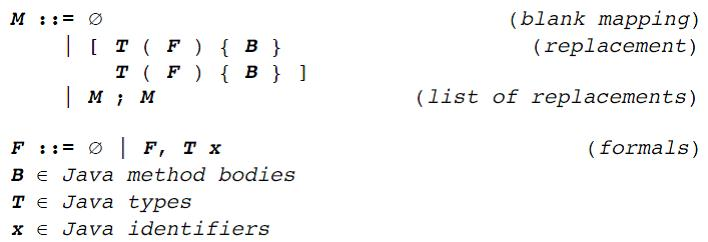
\includegraphics[width=8.5cm]{one}
%    \caption{Syntax of twinning}
%    \label{fig-syntax}
%  \end{figure}

Twinning is a rule-based language for adapting programs between
alternative APIs. The design goal of Twinning is to be easy to use
while allowing a reasonable set of adaptation tasks to be
specified. 
%Figure~\ref{fig-syntax} shows the syntax of Twinning. 
A Twinning program basically consists of a set of replacement rules 
in the form of
\[
\begin{array}{ll}
~[ \\
\tt\quad T_{10} (T_{11}~x_1, \ldots, T_{1n}~x_n)~\{~ \mbox{{\bf return }javaExp}_1;~\}\\
\tt\quad T_{20} (T_{21}~y_1, \ldots, T_{2n}~y_n)~\{~ \mbox{{\bf return }javaExp}_2;~\}\\
~]
\end{array}
\]
which means (1) $T_{1i}$ will be replaced by $T_{2i}$ for all $i$ (the
set of pairs $[T_{1i}, T_{2i}]$ from all replacement rules are called
a \emph{type mapping}); (2) $x_i$ is a meta variable that will match a
Java expression of type $T_{1i}$ in the source code and instantiates
$y_i$ with that expression;
(3)
$\mbox{javaExp}_1$, which is a Java expression of type $T_{10}$ that uses meta 
variables $x_1\ldots x_n$, will be used to match Java expressions, and these
expressions will be replaced by $\mbox{javaExp}_2$ of type $T_{20}$, where the meta
variables $y_i$ are instantiated with the matched expressions by $x_1\ldots x_n$
% Java expressions matched by
% $\mbox{javaExp}_1$ that uses meta variables $x_i$ and has type
% $T_{10}$ will be replaced by Java expression
% $\mbox{javaExp}_2$ that uses meta variables $y_i$ and has type
% $T_{20}$
\footnote{Strictly speaking, Twinning also allows replacing a
  block of statements rather than a single expression. For the ease of
  presentation, we shall only consider expression replacement in this
  paper. All discussions apply to statements replacement as well.}.
%
%
%\begin{example}[Replacement Rule]
%  \rm

As a simple example, consider the following replacement rule
\begin{quote}
\begin{lstlisting}[numbers=left]
[ 
 Enumeration(Hashtable x) 
  {return x.elements();}
 Iterator(HashMap x) 
  {return x.values().iterator();} 
]
\end{lstlisting}
\end{quote}
which will match any call to \code{elements} in class \code{Hashtable}, and replace it by a call to \code{values().iterator()} in class \code{HashMap}. 
%The expression after the
%first \code{return} in line 3 will be used to match an expression in
%the Java code, where the variable \code{x} is a meta variable used to
%match a Java variable of type \code{Hashtable}. The expression after
%the \code{return} in line 5 will be used to replace any matched
%expression, where the meta variable \code{x} will be replaced by the
%name of the matched Java variable. The return type \code{Enumeration} in line
%2 and the return type \code{Iterator} in line 4 are used to declare the
%return types of the expressions to ease the type analysis of the
%language.
For instance, given the following piece of code,
\begin{quote}
\begin{lstlisting}
void f(Hashtable t) {
  Enumeration e = t.elements():
  ...
}
\end{lstlisting}
\end{quote}
the replacement rule will produce the following piece of code, where
the meta variable \code{x} in the replacement rule matches the expression \code{t}.
\begin{quote}
\begin{lstlisting}
void f(HashMap t) {
  Iterator e = t.values().iterator():
  ...
}
\end{lstlisting}
\end{quote}
%\myendup
%\end{example}

%Besides replacing method calls, Twinning also collect a type mapping
%from all replacements, and the type mapping is collected from the
%return types of the replacement and the types of the pointwisely
%corresponding meta variables. The above example declares two pairs for
%the type mapping. One is from the return type, mapping \code{Enumeration} to
%\code{Iterator}, and the other one is from the declaration of the meta
%variable $x$, mapping \code{Hashtable} to \code{HashMap}. After
%collecting the type mapping, Twinning will replace the type uses in
%the Java source code according to the type mapping. In this case, all
%type occurrences of \code{Enumeration} in the Java code will be
%replaced as \code{Iterator}, and all type occurrences \code{Hashtable}
%will be replaced as \code{HashMap}. 


Twinning mainly checks two conditions to avoid introducing new type errors
in the code. First, Twinning requires each replacement must be
well typed under the typing rules of Java. In this way, we can
ensure the replacement of expressions does not introduce new type 
errors. Second, Twinning requires that one type is only mapped to
one type in the type mapping (i.e., one type cannot be mapped to different types by 
replacement rules). This condition ensures that the replacement of
types can be correctly performed.

Unfortunately, these two conditions cannot fully ensure type safety. 
First, \yxmodifyok{Twinning cannot guarantee subtyping preservation.}{type errors may be
introduced when subtyping relations are
involved.} 
%
% Though the checking rules of Twinning are quite reasonable, these
%rules alone cannot ensure type safety. 
To see this, consider a
practical example to adapt
programs from Java Swing API to SWT API~\cite{icsm2010}, where 
 the correspondences between types of
the two APIs are summarized in Figure~\ref{fig-swingtoswt},
and the following presents part of the rules for replacing 
type constructors to their counterparts.
\begin{quote}
\begin{lstlisting}
[ 
 Container () {return new Container();}
 Composite () 
  {return new Composite(new Shell(), 0);}
]

[ JList () { return new JList(); } 
  List  () { return new List(); } ]
\end{lstlisting}
\end{quote}
%
%[ JFrame () { return new JFrame(); }
%  Shell () { return new Shell(); } ]
%These rules replaces  Some constructors on the SWT side have more parameters
%than those in Swing, so we provide default values for these constructors.
% \noindent PAR and N are default values provided for constructor of class Composite.
% It seems right while using these rules to update clients with API Swing, 
% but consider following statement in a type-safety client program:
The typing problem happens if we apply the above rules to the following piece of code:
\begin{quote}
\begin{lstlisting}[language=Java]
Container x = new JList();
\end{lstlisting}
\end{quote}
Clearly, it will yield the code
%
%If we transform this statement with rules above, it will replace the
%constructor call to \code{JList()} with a call to \code{List()}, and
%replace \code{Container} with \code{Composite}. The transformed client
%code is shown as follows.
\begin{quote}
\begin{lstlisting}[language=Java]
Composite x = new List(); 
\end{lstlisting}
\end{quote}
which actually contains a type error:
JList is a subtype of Container, but List is not a subtype of
Composite, so we cannot assign a \code{List} object to a
\code{Composite} variable. This example shows that, although the two
conditions used in Twinning ensure the replacement of expressions and the
replacement of types are correct by themselves, the {\em intersection} of
the two replacements would introduce type errors.

\begin{figure}
    \centering
    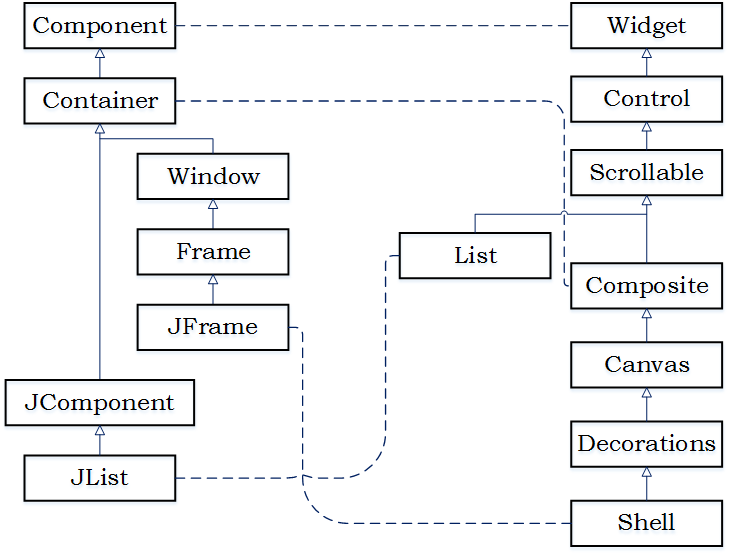
\includegraphics[width=7cm]{swingtoswt}
    \caption{Swing and SWT Type Mapping} 
    \label{fig-swingtoswt}
\end{figure}

% . The cast of type List
% to type Composite is a wrong cast, so the rules above cannot preserve the type correctness.
% In our work, these rules will be excluded.

%The above example shows that the constraints of twinning is not enough to preserve the type
%correctness while updating programs. 

Second, Twinning has no guarantee
% that all components appeared only in the old API are
% fully replaced by components in the new API.
the replacement rules cover all necessary changes.
When there are components appearing only in the old API but are not
transformed by any transformation rule, type errors may be introduced.
% This would introduce type errors when an old component exists in an updated program.
For instance, consider the upgrade of Java SDK from v1.0
to v1.2: class \code{Hashtable} (Figure~\ref{fig:hashtable}) is replaced by
\code{HashMap} (Figure~\ref{fig:hashmap}). For this change, we write a set of 
replacement rules (Figure~\ref{fig:table2map}).
%
%From these rules, we can see method \textit{elements} in class Hashtable
%maps to two methods \textit{values} in class HashMap and \textit{iterator} in
%class Collection. We also require the bodies of these rules can be type checked,
%and the type mapping is a function as twinning. 
To be sure that any program using \code{Hashtable} can be transformed 
in a type-safe way, we must guarantee that all methods and classes in
\code{Hashtable} have their replacements. However, the method \code{contains}
in class \code{Hashtable} has no such replacements in the 
above set of rules. % This means that type-safety requires taking
% account of the difference between the old API and the new API.
%\todo{We can separate the following as the third problem. One reviewer
  %complained that he could not understand our solution to this problem,
  %but I think this is because he missed the problem.} Another more subtle case is that when one replacement declares a type
%change but there is no rule to implement that change. For example, let
%us remove the first rule in Figure~\ref{fig:table2map}. The
%application of the second rule will always introduce a type error
%because the expression matched by \code{x} will never be transformed
%and remains to have type \code{Hashtable}.

\begin{figure}
\begin{lstlisting}[language=java]
class Hashtable {
    Enumeration elements() { }
    boolean contains(Object v) { }
    ...
}
class Enumeration {
    ...
}
\end{lstlisting}
\caption{Hashtable API}
\label{fig:hashtable}
\end{figure}
    % boolean hasMoreElements() { }
    % Object nextElement() { }

\begin{figure}
\begin{lstlisting}[language=java]
class HashMap {
    Collection values() { }            
    boolean containsValue(Object v) { }
    ...
}
class Collection {
    Iterator iterator() { }
    ...
}
class Iterator {
    ...
}
\end{lstlisting}
\caption{HashMap API}
\label{fig:hashmap}
\end{figure}
    % boolean hasNext() { }
    % Object next() { }


\begin{figure}
\begin{lstlisting}
[ Hashtable () { return new Hashtable();}
  HashMap () { return new HashMap(); } ]

[ Enumeration (Hashtable x) 
    { return x.elements(); }
  Iterator (HashMap x) 
    { return x.values().iterator(); } ]
\end{lstlisting}
\caption{Replacement Rules From Hashtable to HashMap}
\label{fig:table2map}
\end{figure}

% [ boolean (Enumeration v) 
%     { return v.hasMoreElements(); }
%   boolean (Iterator v) 
%     { return v.hasNext(); } ]

% [ Object (Enumeration v) 
%     { return v.nextElement(); }
%   Object (Iterator v) 
%     { return v.next(); } ]

In summary, the conditions of Twinning are not
enough to ensure type-safety of the transformation program. We need
the additional conditions to prevent the above two cases. For the first
case, we need to ensure that  the type mapping does not break the
subtyping relations. For the second case, we need to ensure the
replacements cover the full API changes. Putting them together with
the original two conditions from Twinning, we
have the following four conditions.
\begin{itemize}
\item For each code snippet introduced in a replacement rule, the code
  snippet itself must be well typed.
\item The type mapping must form a function, i.e., no type in the
  source API is mapped to two or more types in the target API.
\item The type mapping must preserve the subtyping relation. If $X$ is
  a subtype of $Y$ in the source API and $m$ is the mapping, $m(X)$
  must be a subtype of $m(Y)$ in the target API.
\item % For any method $m$ or field $f$ in the source API, if $m$ or $f$ does
  % not exist in the target API, there must exist a replacement rule
  % matching $m$ or $f$.
  The replacement rules must cover all type changes between the source
  API and target API, 
  %\todo{we should also separate the rest part as a
    %new rule, and change all text in the paper accordingly.(4 rules $\rightarrow$
  %5 rules)} 
  as well as any type changes declared in the type mapping.
\end{itemize}

It will be interesting to see later that these four conditions are
sufficient to ensure type safety. However, as Twinning is presented
informally in the original publication \cite{twinning}, to reason about
type safety,
we need to first build a formal model of the Twinning semantics. A
particular challenge of presenting this formal model is to understand
how the replacement rules can be sequentially applied. For example, to
transform the following piece of code
\begin{quote}
\begin{lstlisting}
new Hashtable().elements()
\end{lstlisting}
\end{quote}
into
\begin{quote}
\begin{lstlisting}
new HashMap().values().iterator()
\end{lstlisting}
\end{quote}
we need to begin with the second rule in
Figure~\ref{fig:table2map} to replace ``\code{elements()}'' and then apply
the first rule to replace ``\code{new Hashtable()}''. If we begin with the
first rule, we shall get an expression
\begin{quote}
\begin{lstlisting}
new HashMap().elements()
\end{lstlisting}
\end{quote}
where the second rule cannot be applied because ``\code{new
  HashMap()}'' has a type \code{HashMap} that cannot be matched by the meta
variable \code{x} of type \code{Hashtable}. In other words, the
transformation is not \emph{confluent} since applying the rules in
different orders gives us different results.

A related issue is that some sequences of rule applications may be
infinite. For example, let us consider the following rule.
\begin{quote}
\begin{lstlisting}
[A (A x) {return x.a();} 
 A (A x) {return x.a().a();]
\end{lstlisting}
\end{quote}
Since the target side of the right also contains the call to
\code{a()}, the rule can be applied again after the transformation,
forming a \emph{non-terminating} transformation.
A terminating and confluent transformation is called a {\em
  convergent} transformation.
A well-formed transformation language should always produce 
convergent transformations. 
However, the publication on Twinning
\cite{twinning} provides no information how Twinning deals with these
issues.

Another usability issue of Twinning is that Twinning allows only exact
type matching, i.e., a meta variable of type $T$ matches a Java
expression only when the expression has exactly type $T$ but not a subtype of $T$. This design eases the
analysis as we can infer all type changes from the type mapping, but
also makes transformation more difficult to write. For example, in
Java v1.0 class \code{Properties} is a sub class of \code{Hashtable},
and thus any call to \code{Properties.elements()} should be
transformed in the same way as \code{Hashtable.elements()}. However,
the second rule in Figure~\ref{fig:table2map} does not apply to calls
to \code{Properties.elements()} because the meta variable \code{x}
has type \code{Hashtable}. As a result, for any replacement rule for a
class $\tt C$, we need to repeat the rule for each sub class of $\tt C$, which
is quite tedious.

To overcome this problem, we design a new language, SWIN (Safe
tWINning). SWIN is based on Twinning but with the following
differences.
\begin{itemize}
\item SWIN has full formal semantics.
  \item SWIN has more flexible rule
application behavior, allowing a meta
variable to match an expression of its sub type.

\item SWIN is convergent. A well typed SWIN program can act on any 
    Java program confluently and free from non-terminating problems.
%\item SWIN employs a normal order evaluation semantics. First, the evaluation rules visit
    %a term leftmost and outermost. After performing the transformation on that term, the evaluation 
    %rules recursively visit the sub terms of the term, and for each visit, the transformation
    %will be applied on the original sub terms, and produce the transformation result by combining
    %the transformed sub terms. This strategy guarantees that the evaluation process is free from
    %confluence and termination problems, as each program element is transformed at most once.
%\item SWIN employs a ``match all, transform once'' semantics. The
  %source program is first matched by the rules and then the
  %replacements of all matches are performed simultaneously. In this way we
  %have no sequential application of rules, effectively avoiding the
  %confluence and termination problem.
%   employs
% a strict top-down order of rule applications, ensuring the
% transformation to be confluent and terminating.
\item SWIN
includes a set of type checking rules checking the four conditions presented
above.
\end{itemize}
In the following sections we shall introduce SWIN formally and
present our proof of type safety.

%These rules will serve as the basis 
%of our new type-safe Java program adaptation framework.

% . In the next section we shall formally show that they are. 


%  Now the question is whether the four rules are enough to ensure type
%  safety. In the next section we shall formally show that they are. 

% From these examples, we can see that invalid or incomplete rules in twinning 
% may introduce type-errors
% while updating client programs. In our paper, we should exclude invalid rules, 
% and assure the all the valid rules in SWIN can preserve the type
% correctness while updating any type-safety programs. 
% In our paper, we give a set of properties that a type safe rule
% should satisfy with, and we call these properties are type safe properties 
% (short for safe properties). There are mainly three properties that rules
% should satisfy with. Next, we will informally and briefly explain these two cases. 

% Consider a rule:
% \begin{align*}
%     [ \quad &T_{1} \quad ( \bar{F} \quad \bar{x} ) \quad \{ \quad B_{1} \quad \} \\
%      &T_{2} \quad ( \bar{G} \quad \bar{y}) \quad \{ \quad B_{2} \quad \} \quad]
%  \end{align*}
%  In rules above, $\bar{F}\; \bar{x}$ is short for $F_{1}\;x_{1},F_{2}\;x_{2},\cdots,F_{n}\;x_{n}$,
%  same as $\bar{G}\;\bar{y}$. 

%  \begin{itemize}
%      \item In rule checking, first, it require that all the variables in
%  $B_{1}$ should be binded with $\bar{x}$, and all the $\bar{x}$ are apperance in $B_{1}$. Second, it 
%  need to assure that $B_{1}$ is a single body, 
%  it means there is no more than one method invoke in $B_{1}$.

%     \item We also collect the type mapping as twinning, and these type mapping should be a 
%         funtion. All the methods in rules should cover all the methods in class appeared in rules, and
%         for the methods in rules should type-safety according the definition of APIs. For any method
%         not in rules, there should be a method in mapped class with same name, and the type of
%         parameters and return value should satisfy the type mapping.

%     \item The last properties is about inheritance. For the inheritance of classes in former API, 
%         these relationship cannot be removed in new API of between any two classes after updated, and
%         the adding of relationship between classes is allowed.
% \end{itemize}


%%% Local Variables: 
%%% mode: latex
%%% TeX-master: "pepm-15"
%%% End: 

%\section{Motivating Example}
In this section, we first give a brief description of update language twinning. Then, we
will give some examples to show why twinning cannot preserve the type correctness while
updating programs. Finally,
we will informally present an overview of our work.
\label{example}
\begin{figure}
    \centering
    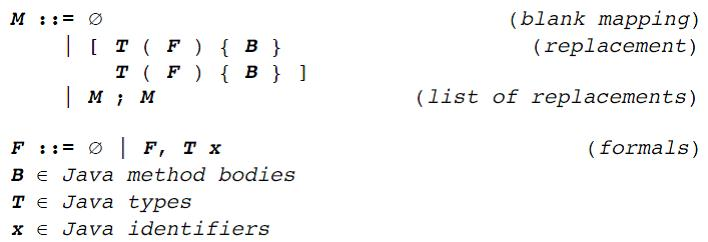
\includegraphics[width=8.5cm]{one}
    \caption{Syntax of twinning}
    \label{fig-syntax}
\end{figure}

\begin{figure}
    \centering
    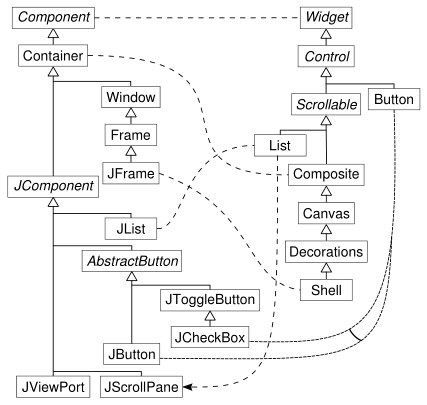
\includegraphics[width=7.5cm]{two}
        \caption{One option for Swing and SWT type mapping}~\cite{icsm2010}
    \label{fig-swingtoswt}
\end{figure}
Twinning is a rule-based language which describes the program modification to adapt to 
a new API. 
Twinning is very simple and easy to learn, as well as useful for its
powerful expressive ability.
Figure \ref{fig-syntax} shows the syntax of twinning which is restricted to the specification of single 
replacements. The main body of twinning is \textit{mapping}. A mapping M is a list of replacements, and
a replacement:

\begin{align*}
    [ &\quad T_{1} \quad ( \quad F_{1} \quad ) \quad \{ \quad B_{1} \quad \} \\
      &\quad T_{2} \quad ( \quad F_{2} \quad ) \quad \{ \quad B_{2} \quad \} \quad]
\end{align*}

\noindent consists of two nameless procedures, means replace $B_{1}$ with 
$B_{2}$. 
$T_{1}$ shows the type of $B_{1}$, and type list $F_{1}$ illustrates the
type of all the variables in body $B_{1}$. Similar with $B_{2}$. 
Type list of $F_{1}$ is point-wise related to the type list of
$F_{2}$. When a replacement was applied in a Java program, $B_{1}$ will match a code block 
(usually is a expression), then replace the code block with $B_{2}$.
Next, we will illustrate how twinning try to preserve type correct.


%详细说明twinning的type checking
First, twinning computes the type-mapping between former API and new API
According to collect type pairs from rules:
\begin{align*}
    &TypeMapping(\phi) = \phi \\
    &TypeMapping([T_{r}\,(T_{1}\,x_{1},\cdots,T_{n}\,x_{n})\; \{\,B\,\} \\
    &\quad\quad\quad\quad\quad\quad\quad T'_{r}\,(T'_{1}\,y_{1},\cdots,T'_{n}\,y_{n})\; \{\,B'\,\}]) \\
    &\quad={(T_{r},T'_{r}),\,(T_{1},T'_{1})\,\cdots,(T_{n}, T'{n})}\\
    &TypeMapping(M;M')\\
    &\quad =TypeMapping(M)\cup TypeMapping(M')
\end{align*}

Twinning demands that the type mapping is a function: $\forall T_{i}$, $\exists$ 
only one $T'_{i}$, that $T_{i}$ map to $T'_{i}$. 
There is a type checking while rules are matching the Java programs.
While a rule is matching a expression,
the types of variable in expression should being matched with type list in a rule
and type of the expression should match return type of the rule. 

We can see that twinning restrict the type mapping as a function and add a type checking while do
the match.
All this seems work good to preserve the type correctness while updating a program, 
but is this really enough to
preserve the type correctness?
Consider the API alternative from Swing to SWT, the inheritance relationship of classes in these two APIs lists in 
Figure \ref{fig-swingtoswt}. In figure \ref{fig-swingtoswt}, all the
mapping of classes is function, so we can use twinning to write rules about updating these classes. 
Some of the rules as follow:

\begin{verbatim}
[ Container () { return new Container(); }
  Composite () { return new Composite(PAR, N); } ]

[ JList () { return new JList(); } 
  List () { return new List(); } ]

[ JFrame () { return new JFrame(); }
  Shell () { return new Shell(); } ]
\end{verbatim}

\noindent PAR and N are default values provided for constructor of class Composite.
It seems right while using these rules to update clients with API Swing, 
but consider following statement in a type-safety client program:

\begin{lstlisting}[language=Java]
Container x = new JList();
\end{lstlisting}

\noindent If we update this statement with rules above, it will introduce a type error 
in the updated client.
The updated client code will be:
\begin{lstlisting}[language=Java]
Composite x = new List(); 
\end{lstlisting}
JList is a subtype of Container, but List is not a subtype of Composite. The cast of type List
to type Composite is a wrong cast, so the rules above cannot preserve the type correctness.
In our work, these rules will be excluded. 

The above example shows that the constraints of twinning is not enough to preserve the type
correctness while updating programs. Another example is about using HashMap as an alternative
class of class Hashtable. Part of methods in class Hashtable and the related class of Hashtable
as follows:

\begin{lstlisting}[language=java]
class Hashtable {
    Enumeration elements() { }
    boolean contains(Object v) { }
    Enumeration keys() { }
    ...
}
class Enumeration {
    boolean hasMoreElements() { }
    Object nextElement() { }
    ...
}
\end{lstlisting}

In this API alternative,
Class Hashtable maps to HashMap, and class Enumeration maps to class Iterator. The methods mapping
to methods listing above in HashMap and Iterator are as follows:

\begin{lstlisting}[language=java]
class HashMap {
    Collection values() { }            
    boolean containsValue(Object v) { }
    Set keySet() { }
    ...
}
class Collection {
    Iterator iterator() { }
    ...
}
class Set { 
    Iterator iterator() { }
    ...
}
class Iterator {
    boolean hasNext() { }
    Object next() { }
    ...
}
\end{lstlisting}

We can use SWIN to describe the mapping rules of this API alternative, the mapping rules:

\begin{verbatim}
[ Hashtable () { return new Hashtable(); }
  HashMap () { return new HashMap(); } ]

[ Enumeration (Hashtable x) { return x.elements(); }
  Iterator (HashMap x) { return x.values().iterator(); } ]

[ boolean (Enumeration v) { return v.hasMoreElements(); }
  boolean (Iterator v) { return v.hasNext(); } ]

[ Object (Enumeration v) { return v.nextElement(); }
  Object (Iterator v) { return v.next(); } ]
\end{verbatim}

From these rules, we can see method \textit{elements} in class Hashtable
maps to two methods \textit{values} in class HashMap and \textit{iterator} in
class Collection. We also require the bodies of these rules can be type checked,
and the type mapping is a function as twinning. But our paper want to make sure
all the clients using Hashtable should be update type safely. These rules are
not enough for our goal, we should assure that all the methods and classes in
Hashtable have replacements, such as methods \textit{contains} and \textit{keys} in class
Hashtable. Adding this condition, we can assure the clients
can be safely updated.


From these examples, we can see that invalid or incomplete rules in twinning 
may introduce type-errors
while updating client programs. In our paper, we should exclude invalid rules, 
and assure the all the valid rules in SWIN can preserve the type
correctness while updating any type-safety programs. 
In our paper, we give a set of properties that a type safe rule
should satisfy with, and we call these properties are type safe properties 
(short for safe properties). There are mainly three properties that rules
should satisfy with. Next, we will informally and briefly explain these two cases. 

Consider a rule:
\begin{align*}
    [ \quad &T_{1} \quad ( \bar{F} \quad \bar{x} ) \quad \{ \quad B_{1} \quad \} \\
     &T_{2} \quad ( \bar{G} \quad \bar{y}) \quad \{ \quad B_{2} \quad \} \quad]
 \end{align*}
 In rules above, $\bar{F}\; \bar{x}$ is short for $F_{1}\;x_{1},F_{2}\;x_{2},\cdots,F_{n}\;x_{n}$,
 same as $\bar{G}\;\bar{y}$. 

 \begin{itemize}
     \item In rule checking, first, it require that all the variables in
 $B_{1}$ should be binded with $\bar{x}$, and all the $\bar{x}$ are appearance in $B_{1}$. Second, it 
 need to assure that $B_{1}$ is a single body, 
 it means there is no more than one method invoke in $B_{1}$.

    \item We also collect the type mapping as twinning, and these type mapping should be a 
        function. All the methods in rules should cover all the methods in class appeared in rules, and
        for the methods in rules should type-safety according the definition of APIs. For any method
        not in rules, there should be a method in mapped class with same name, and the type of
        parameters and return value should satisfy the type mapping.

    \item The last properties is about inheritance. For the inheritance of classes in former API, 
        these relationship cannot be removed in new API of between any two classes after updated, and
        the adding of relationship between classes is allowed.
\end{itemize}


\begin{section}{Syntax and Semantics of Core SWIN}
\label{tw-fj}

Before explaining full SWIN for Java, which will
be discussed in Section~\ref{sec:extension}, we start with 
core SWIN for Featherweight Java~\cite{fj},
a known minimal core of Java. % Strictly speaking, 
% the transformation language for Featherweight Java is \emph{core} SWIN, and
% SWIN is for full Java. 
% If there is no confusion, in the follow text, we use
% SWIN for short.
If no confusion will be caused, we shall directly use SWIN to refer core SWIN.
We shall briefly review Featherweight Java, and 
explain the syntax and semantics of our transformation language SWIN for it.

\subsection{Background: Featherweight Java}
Featherweight Java (FJ for short) is a minimal core calculus for Java~\cite{fj}. 
FJ is small enough that a concise proof of type preserving
property is possible while it can be easily extended to full Java.

\begin{figure}[ht]
\begin{align*}
  & \mbox{Class Declaration}\\
  & \qquad\tt CL\ ::=\  \tt class\ C\ extends\ C \{\bar{C}\ \bar{f}; K\ \bar{M}\}\\
  & \mbox{Constructor Declaration}\\
  & \qquad\tt K \ ::=\  \tt C\ (\bar{C}\ \bar{f})\ \{ super(\bar{f}); this.\bar{f}=\bar{f}\}\\
  & \mbox{Method Declaration}\\
  & \qquad\tt M \ ::=\  \tt C\ m(\bar{C}\ \bar{x})\ \{ return\ t;\}\\
  & \mbox{Term}\\
  & \qquad\tt t \ ::=\  \tt x\ |\ t.f\ |\ t.m(\bar{t})\ |\ new\ C(\bar{t})\ |\ (C)\ t
\end{align*}
\caption{Syntax of Featherweight Java}
\label{fj-syntax}
\end{figure}
Figure~\ref{fj-syntax} shows the syntax of FJ.
The class declaration 
\[
\tt class\ C\ extends\ D\ \{\bar{C}\ \bar{f};\ K\ \bar{M}\}
\]
introduces a class named \verb|C| with superclass \verb|D|. The class has fields $\tt\bar{f}$ with types $\tt\bar{C}$,
a single constructor \verb|K|, and a suite of methods $\tt\bar{M}$.
%In the syntax of FJ, it abbreviate operations on pairs of
%sequences in the obvious way, 
In the formal notations, we use the bar notation adopted by Pierce~\cite{tpl} for repetitive elements: 
$\bar{a}$ to indicate a vector $a$,
and all operations defined on single values expand componentwisely to
vectors. For example, let $x_i$ be the $i$th element in $\bar{x}$, we
have $\bar{a}<\bar{b}$ is equal to $\forall i.\ a_i < b_i$ and $\bar{a}
\in S$ is equal to $\forall i.\ a_i \in S$.
Here, we write $\tt \bar{C}\ \bar{f}$ for $\tt C_{1}\,f_{1},\cdots,
C_{n}\,f_{n}$, where $\tt n$ is the length of $\tt\bar{C}$ and $\tt\bar{f}$.
Similarly, $\tt \bar{M};$ denotes $\tt M_1;\cdots ;M_n$, and $\tt \bar{M}$ 
denotes $\tt M_1\cdots M_n$.

The constructor declaration 
\[
\tt C(\bar{C}\,\bar{f})\{super(\bar{f});\,this.\bar{f}=\bar{f};\}
\]
defines the way to initialize a Java object, including a call to superclass constructor and assignments to class fields.

The method declaration 
\[
\tt C\ m(\bar{C}\ \bar{x})\{\ return\ t;\ \}
\]
introduces a method named $\tt m$ with return type $\tt C$ and
parameters $\tt \bar{x}$ of types $\tt\bar{C}$. The body of the method
is just a single term $\tt return\ t$.
%, and $\bar{x}$ is definition of
%bounded variables in $\tt t$.

There are only five terms in FJ, variable $\tt x$, field access $\tt
t.f$, method invocation $\tt t.m(\bar{t})$, object creation $\tt new\ 
C(\bar{e})$, and cast operation $\tt (C)e$. 
%There are no assignments,
%interfaces, overloading, messages to super, null pointers, base types,
%abstract method declarations, inner classes, etc.  
The  key
simplification in FJ is the omission of assignment. This implies that
an object's field is initialized by its constructor and never
changed afterwards. This restricts FJ to a ``functional'' fragment of
Java.
%, but is computationally complete as it is easy to encode
%lambda-calculus into it.

The typing rules of FJ are the same as those of plain
Java. One exception is that FJ does not support method
overloading. We refer the reader to the original paper~\cite{fj} and
Appendix~\ref{sec:FJTyping} for the typing rules. 

% \paragraph{APIs in Featherweight Java}
% \clmodify{}{Add this new section to introduce API in FJ}\todo{Revise this}

% As Featherweight Java is not a modular programming language,
% we define API in FJ as a bunch of class declarations in a FJ program and these class declarations are well type without refer to other class declarations.
% So an FJ program $\tt p=\bar{CL}$ can be divided into two parts: $\tt\overline{CL}_{API}$ and $\tt\overline{CL}_{client}$ (i.e. $\tt p = \overline{CL}_{API}~\overline{CL}_{client}$). 
% A transformation on a FJ program is to transform $\tt\overline{CL}_{client}$ and then replace $\tt\overline{CL}_{API}$ with new API class declarations $\tt\overline{CL}'_{API}$.
% The formal definition of the APIs in typing rules will be present later together with SWIN type checking systems.


\subsection{Core SWIN% : A Type-Safe Transformation Language
}

% SWIN is based on Twinning but with formal and more flexible
% semantics, which will be discussed here.
% In particular, SWIN employs a strict top-down order of rule
% applications, ensuring the transformation to be confluent and
% terminating. Furthermore, as will be seen in Section \ref{tw-type} later,
% SWIN also includes a set of typing
% rules checking the four conditions presented above. In the following
% sections we shall introduce SWIN formally and present our proof of
% type safety.
In this subsection we describe the syntax and evaluation rules of
SWIN formally. The type checking rules and the proof of type-safety property will be
presented in Section~\ref{tw-type} later.

\subsubsection{Syntax}

% SWIN is an update language specifying 
% how to transform client programs using old APIs to those using new APIs. 
The formal definition of SWIN is presented
in Figure~\ref{syntaxofuc}. Simiarly to Twinning, a SWIN program $\tt\Pi$ is a set of 
transformation rules, and a transformation rule ($\tt\pi=(\bar{d})\ [l:C_l\ \rightarrow\ r:C_r]$) consists of three
parts: 1) meta variable declarations ($\tt \bar{d}$), 2) left hand side source
code pattern ($\tt l$) and 3) right hand side target code pattern ($\tt r$). 
Source code pattern $\tt l$ will be used to match an expression in old client program,
and target code pattern $\tt r$ is an FJ term use a new API with meta-variables bounded in $\tt d$
which is used to generate updated client code. And the variable declaration part
($\tt d=x:A\hookrightarrow B$) associates a metavariable with its type migration information: $\tt x$ is of type $\tt A$ in $\tt l$ and of type $\tt B$ in $\tt r$.

\begin{figure}
\begin{align*}
  \tt \Pi \quad ::=\quad  &\tt  \{\bar\pi\}                     &\text{Transformation program}\\
  \tt \pi \quad ::=\quad  &\tt  (\bar{d})\ [l\ \rightarrow\ r]    &\text{Rule}\\
  \tt d   \quad ::=\quad  &\tt  x:C_1\hookrightarrow C_2          & \text{Variable declaration}\\
  \tt l   \quad ::=\quad  &\tt  x.f ~ | ~ new\ C(\bar{x}) ~|~ x.m(\bar{x})  & \text{Code pattern}\\
  \tt r   \quad ::=\quad  &\tt  t                                 &\text{FJ term}
\end{align*}
%Variables in $\tt r$ are meta-variables bounded by the variable definition in $\pi$.
\caption{Syntax of SWIN}
\label{syntaxofuc}
\end{figure}

An informal explanation of the rule can be seen from its correspondence 
with the replacement rule in Section \ref{sec:examples}. 
For example, the mapping rule
\[
\tt
\pi=(x:A\hookrightarrow
L,y:B\hookrightarrow M)\ [\ x.m(y):C \rightarrow x.h(y):D\ ]
\]
can be seen as the following replacement rule:
\begin{quote}
\begin{lstlisting}
[ 
 C (A x, B y) { return x.m(y); }
 D (L x, M y) { return x.h(y); }
]
\end{lstlisting}
\end{quote}
%The first part $\tt x.m(y)$ means that the source pattern is a Java
%term of invocation.  The method name is $\tt m$ and it is a method of
%object $\tt x$, which is an object of class $\tt A$ according to the
%variable declaration $\tt x:A\hookrightarrow L$ part of the rule.  The
%declaration $\tt y:B\hookrightarrow M$ and the appearence of $\tt y$
%in $\tt x.m(y)$ indicates the method $\tt m$ has only one argument of
%type $\tt B$.  
Now if there is a client source code term $\tt
(new\ A()).m(new\ B())$, the rule will match the term as \verb|x| binds to
$\tt new\ A()$, \verb|y| binds to $\tt new\ B()$, and the method name
$\tt m$ matches the method name in the term. It results in that the updated term
$\tt (new\ A()).h(new\ B())$ is of type $D$.
Note that this rule 
does not match the term $\tt (new\ C()).m(new\ B())$, as the type
of the variable $\tt x$ (type $\tt A$) does not
match the type of the term $\tt new\ C()$ (type $\tt C$).  
%The third
%part $\tt x.h(y)$ of $\pi$ is the target code pattern, which will be
%used to generate new client code with meta-variable substitution and
%it will be introduced in the next part.  
%
% One thing we need to take care about is the variable declaration part
% of a rule $\tt \pi$.  
% Note also that in a mapping rule, there may be variables
% appearing in both source code pattern and target code pattern, and all
% these variables should be specified in the variable declaration part.
% A declaration for $x:A\hookrightarrow B$ means that in source code
% pattern $\tt l$, $\tt x$ has type $\tt A$ and in target code pattern
% $\tt r$, $\tt x$ has type $\tt B$, and these $\tt x$ are exactly the
% same. It is defined in this way as when we apply the rule to a
% piece of client code, a matching of source code pattern will generate
% a substitution of $\tt x\rightarrow t$, which will be used to instantiate
% $\tt x$ in target code pattern with $\tt t$ and generate new client
% code.

To ensure convergence, we do not allow the left hand sides of
two rules to match the same method or the same constructor. In this
way we can ensure one term is matched by at most one rule, resulting
in a unique result after transformation.
% Furthermore, for the ease of presentation, we do not allow a rule 
% to replace a field access in the SWIN for FJ, 
% such as replacing \code{t.f} with \code{t.m()}.
% This feature can be easily implemented by treating a field as a method
% without parameter in FJ, because FJ does not allow
% the writing of an API field in the user code while the initialization
% of a field is inside an API itself and does not need to be
% transformed. Yet in full Java, supporting fields needs some more work,
% as will be discussed in Section~\ref{sec:extension}.


\subsubsection{Semantics: Evaluation Rules}

We assume that an FJ program, which is a set of class declarations, can be divided into two parts: 
$\tt\{\overline{CL}_{API}\}$ and $\tt\{\overline{CL}_{client}\}$,
where $\tt\overline{CL}_{API}$ is the source API,
consisting of class definitions that are
type-correct by themselves; $\tt\overline{CL}_{client}$ is the client
program to be transformed, consisting of class definitions that depends on $\tt\overline{CL}_{API}$. A
transformation on an FJ program is to apply the transformation rules on 
$\tt\overline{CL}_{client}$ to get $\tt\overline{CL}'_{client}$, and then replace $\tt\overline{CL}_{API}$
with the target API $\tt\overline{CL}'_{API}$, such that
$\tt\overline{CL}'_{API}$ and $\tt\overline{CL}'_{client}$ form a
type-correct program. 

In formal notations, we define $\tt API$ to denote $\{~\overline{CL}~\}$, and operations on $\tt API$s are naturally set operations (e.g. $\tt API_1-API_2$ is set substraction, which will exclude class declarations in $\tt API_2$ from $\tt API_1$). In particular, we use the notation $\tt API_s$ to denote the
source API, $\tt\overline{CL}_{API}$, and $\tt API_d$ to denote the target
API, $\tt\overline{CL}'_{API}$, respectively. 

% As Featherweight Java is not a modular programming language,
% we define API in FJ as a bunch of class declarations in a FJ program and these class declarations are well type without refer to other class declarations.
% So an FJ program $\tt p=\bar{CL}$ can be divided into two parts: $\tt\overline{CL}_{API}$ and $\tt\overline{CL}_{client}$ (i.e. $\tt p = \overline{CL}_{API}~\overline{CL}_{client}$). 
% A transformation on a FJ program is to transform $\tt\overline{CL}_{client}$ and then replace $\tt\overline{CL}_{API}$ with new API class declarations $\tt\overline{CL}'_{API}$.
% The formal definition of the APIs in typing rules will be present later together with SWIN type checking systems.



\begin{figure*}[htb!]
\begin{center}
\AXC{$\tt CL=class\ C_{1}\ extends\ C_2\ \{\ \bar{C}\ \bar{f};\ K\ \bar{M}\ \}$}                             \RightLabel{~(E-DECLARATION)}
\UIC{$\tt \Pi(CL)= class\ \Pi(C_1)\ extends\ \Pi(C_2)\ \{\ \Pi(\bar{C})\ \bar{f};\ \Pi(K)\  \overline{\Pi(M)}\ \}$}
\DP
\end{center}
\vspace{2pt}

\begin{center}
\AXC{$\tt K=C_1\ (\bar{C}_2\ \bar{f}_2)\ \{super(\bar{f}_3);\ this.\bar{f}_i=\bar{f}_j\}$}                             \RightLabel{~(E-CONSTRUCTOR)}
\UIC{$\tt \Pi(K)=\Pi(C_1)\ (\Pi(\bar{C}_2)\ \bar{f}_2)\ \{super(\bar{f}_3);\ this.\bar{f}_i=\bar{f}_j\}$}
\DP
\end{center}
\vspace{2pt}

\begin{center}
\AXC{$\tt M=C_1\ m(\bar{C}\ \bar{x})\ \{return\ t;\}$}                             
\RightLabel{~(E-METHOD)}
\UIC{$\tt\Pi(M)=\Pi(C_1)\ m(\Pi(\bar{C})\ \bar{x})\ \{return\ \Pi(t);\}$}
\AXC{$\tt C_0\hookrightarrow C_1\in \mathbf{TypeMapping}(\Pi)$}                             
\RightLabel{~(E-CLASS)}
\UIC{$\tt \Pi(C_0)=C_1$}
\noLine
\BIC{}
\DP
\end{center}
\vspace{2pt}

\begin{center}
\AXC{$\tt \forall C.~C_0\hookrightarrow C\notin \mathbf{TypeMapping}(\Pi)$}
\RightLabel{~(E-ALTER-CLASS)}
\UIC{$\tt \Pi(C_0)=C_0$}
\AXC{}                 \RightLabel{~(E-T-VALUE)}
\UIC{$\tt \Pi(x)=x$}
\noLine
\BIC{}
\DP
\end{center}
\vspace{2pt}

\begin{center}
\AXC{$\tt (x:C_1\hookrightarrow C_2)[~x.f:C\ \rightarrow\ r:D~]\in \Pi$ ~~~~ $\tt\type{t} <: C_1$}                 \RightLabel{~(E-T-FIELD)}
\UIC{$\tt \Pi(t.f)=\tt[~x\rightarrow \Pi(t)~]r$}
\DP
\end{center}
\vspace{2pt}

\begin{center}
\AXC{}      \RightLabel{~(E-T-CAST)}
\UIC{$\tt \Pi((C)\ t)=(\Pi(C))\ \Pi(t)$}
%%% the next rule
\AXC{$\tt (\bar{d})[\ new\ C_0(\ \bar{x}\ ):C\ \rightarrow\ r:D]\in \Pi$}
\noLine
\UIC{$\tt\quad\quad \{~\bar{x}:\overline{C_1\hookrightarrow C_2}~\}\subseteq \bar{d} \quad\quad  \type{\bar{t}_u}<:\bar{C}_1$}               
\RightLabel{~(E-T-NEW)}
\UIC{$\tt \Pi(new\ C_0(\bar{t}_u))=[~\bar{x}\rightarrow \overline{\Pi(t_u)}~](r)$}
\noLine
\BIC{}
\DP
\end{center}
\vspace{2pt}

\begin{center}
\AXC{$\tt  (\bar{d})[\ x_0.m_0(\ \overline{y}\ ):C\ \rightarrow\ r:D]\in\Pi$}
\noLine
\UIC{$\tt \{\bar{y}:\overline{C_1\hookrightarrow C_2},\ x_0:C_3\hookrightarrow C_4\} \subseteq \bar{d} \quad\quad\type{t_0}<:C_3\quad\quad \type{\bar{t}_u}<:\bar{C}_1$}\RightLabel{~(E-T-INVOKE)}
\UIC{$\tt \Pi(t_0.m_0(\bar{t}_u))=[~x_0\rightarrow \Pi(t_0),\ \bar{y}\rightarrow \overline{\Pi(t_u)}~](r)$}
\DP
\end{center}
\vspace{2pt}

\begin{center}
\AXC{$\mbox{\tt no other inference rule can be applied}$}   
\RightLabel{~(E-ALTER-NEW)}
\UIC{$\tt \Pi(new\ C_0(\bar{t}_u))=new\ C_0(~\overline{\Pi(t_u)}~)$}
\DP
\end{center}
\vspace{2pt}

\begin{center}
\AXC{$\mbox{\tt no other inference rule can be applied}$}   
\RightLabel{~(E-ALTER-INVOKE)}
\UIC{$\tt \Pi(t_0.m_0(\bar{t}_u))=\Pi(t_0).m(~\overline{\Pi(t_u)}~)$}
\DP
\end{center}
\vspace{2pt}

\begin{center}
\AXC{$\mbox{\tt no other inference rule can be applied}$}                 \RightLabel{~(E-ALTER-FIELD)}
\UIC{$\tt \Pi(t.f)=\tt\Pi(t).f$}
\DP
\end{center}
\vspace{2pt}
\caption{Evaluation Rules of SWIN}
\label{semanticsofuc}
\end{figure*}

\begin{figure*}
\begin{align*}  
&\tt \mathbf{TypeMapping}([(~\bar{x}:\overline{C_1\hookrightarrow C_2}~)\ [l:C\ \rightarrow\ r:D]]) = \{C\hookrightarrow D\}\cup\{~\overline{C_1\hookrightarrow C_2}~\}\\
&\tt \mathbf{TypeMapping}(\{\bar{\pi}\}) = \bigcup_{\pi}~(\mathbf{TypeMapping}(\pi)) ~~~~~~ \text{(Extract type migration information)}\\
&\tt \mathbf{Decl}(class~C~extends~D~\{...\}) = C   ~~~~~~
\text{(Extract the declared class name)}
% ~~~~~~
% \AXC{$\tt \vdash_{FJ}^{API_S} t : C$}
% \RightLabel{~(Get the type of a term)}
% \UIC{$\tt {Type}(t)=C$}
% \DP
\end{align*}
\caption{Auxiliary Functions used in Figure~\ref{semanticsofuc} and Figure~\ref{logicrules}}
\label{auxiliarydefofuc}
\end{figure*}

%This part defines rules of how to update Java client code with SWIN code.\par
%informally explained the meaning of mapping rules.
Figure~\ref{semanticsofuc} summarizes the formal semantics of SWIN.
In the rules, $\tt A <: B$ indicates that \code{A} is a subtype of \code{B}. A transformation program $\tt\Pi$ is formalized as a transformation from 
source code to target code on both types and terms. This transformation consists of the following three steps.

\begin{enumerate}
\item {\em Transformation Promotion}: The first three rules \\(E-DECLARATION, E-CONSTRUCTOR, E-METHOD)
are used to promote $\tt\Pi$ up to types and terms through a class declaration, a
construction definition, and a method definition, respectively.

\item {\em Type Transformation}: The next E-CLASS rule is used to transform source types in the source API to target types in target API
  based on the type mappings defined in $\tt\Pi$. Those types which
  are not involved in type mapping of $\tt \Pi$ will stay the same
  according to the rule E-ALTER-CLASS. An important components of the
  two rules is \textbf{TypeMapping}, which records how types in $\tt
  API_s$ is mapped to $\tt API_d$ by the transformation program, and
  is defined in Figure~\ref{auxiliarydefofuc}.
  
  % The rules for extracting type migration information from $\tt\Pi$ can be referred to \textbf{TypeMapping} in Figure~\ref{auxiliarydefofuc}.

\item {\em Term Transformation}: The rest of the rules are used to
  transform source code terms. As the syntactic definitions in
  Figure~\ref{syntaxofuc} show, an FJ term takes five forms. The form
  $\tt x$ and $\tt (C)t$ are dealt by E-T-VALUE and E-T-CAST,
  respectively, which basically further applies $\Pi$ to sub terms.
  The other three forms are dealt by E-T-FIELD, E-T-NEW, E-T-INVOKE,
  respectively. The three evaluation rules apply matched SWIN transformation
  rules to the current term. In case no rule can be applied,
  evaluation rules E-ALTER-FIELD, E-ALTER-INVOKE, E-ALTER-NEW apply
  $\Pi$ sub terms. In the definitions, we use $\tt Type(t)$ to get the
  type of a term $\tt t$ based on FJ typing rules.
%   ; $\tt\Pi$ is recursively applied to subterms and 
% its rules are used to transform $\tt new\ C_0(\bar{t}_u)$ or $\tt t_0.m_0(\bar{t}_u)$ or $\tt t.f$ whenever possible.
% When reaching $\tt new\ C_0(\bar{t}_u)$, if there is a rule 
% with the source pattern of the form $\tt new\ C_0(\ \bar{x}\ )$ and the type of $\tt \bar{t}_u$ is a subtype
% of that of $\tt \bar{x}$, it will apply the rule on the term by replacing meta-variables $\tt \bar{x}$ in the target code pattern $\tt r$ by corresponding $\tt \Pi(\bar{t}_u)$ (based on E-T-NEW), otherwise 
% $\tt \Pi$ is recursively applied to its subterm (based on
% E-ALTER-NEW). The cases for $\tt t_0.m_0(\bar{t}_u)$ and $\tt t.f$
% is dealt with similarly.

  
\end{enumerate}

%
%An update body $\tt\Pi$ will transform both types and terms in source code. 
%When we apply $\tt\Pi$ on Java source code,
%generally we have three steps:
%\begin{enumerate}
%\item Match the term with a rule $\tt\pi$ in $\tt\Pi$.
%\item Generate a substitution of meta-variables to Java term based on the matching.
%\item Transform the target code pattern $\tt r$ to Java client code by meta-variables substituti%on.
%\end{enumerate}
%\par

To be concrete, let us see an example. Suppose that we want to switch from 
the old API ($\tt API_s$) to a new one ($\tt API_d$)\footnote{
We omit the API method bodies here as it is not necessary
to see the details of how an API method is implemented;
it is sufficient to show the input types and the return type of each method in API.}
\[
\begin{array}{lll}
\mbox{$\tt API_s=\{class\ A\ \{\ A()\{...\};\ A\ h(A\ a)\{...\};\};\}$}\\
\mbox{$\tt API_d=\{class\ B\ \{\ B()\{...\};\ B\ k(B\ b,B\ c)\{...\};\};\}$}
\end{array}
\]
and we use the following SWIN transformation program
\[
\begin{array}{lll}
\mbox{$\tt\Pi=[\pi_1,\pi_2]$}\\
{\bf where}\\
\quad \mbox{$\tt\pi_1=()\ [\ new\ A() : A \rightarrow new\ B() : B\ ]$}\\
\quad \mbox{$\tt\pi_2=(x:A\hookrightarrow B, u:A\hookrightarrow B)$} \\
\qquad\qquad \mbox{$\tt[\ x.h(u) : A \rightarrow x.k(u,new\ B()) : B\ ]$}
\end{array}
\]
to transform the following source client Java code.
\[
\mbox{$\tt(new\ A()).h(new\ A())$}
\]
The transformation is done as follows.
\[
\begin{array}{llll}
   & \mbox{$\tt \Pi((new\ A()).h(new\ A())$}\\
=  & \reason{by E-T-INVOKE with rule $\pi_2$}\\
   & \mbox{$\tt [x\rightarrow \Pi(new\ A()), u\rightarrow \Pi(new\ A())](x.k(u,new\ B()) )$}\\
=  & \reason{replace $\tt x$ and $\tt u$ in $\tt x.k(u,new\ B())$ }\\
   & \mbox{$\tt \Pi(new\ A()).k( \Pi(new\ A()),new\ B())$}\\
=  & \reason{by E-T-NEW with rule $\pi_1$}\\
   & \mbox{$\tt [~](new\ B()).k( [~](new\ B()),new\ B())$}\\
=  & \reason{ since $\tt [~](new\ B()) = new\ B()$ }\\
   & \mbox{$\tt new\ B().k(new\ B(),new\ B())$}\\
\end{array}
\]
Thus it results in target code $\tt new\ B().k(new\ B(),new\ B())$.

% \subsubsection{Evaluation Property: Convergence}

\smallskip
Our evaluation rules ensure the convergence of any SWIN program, which
is discussed in the following theorem and its proof sketch.
\begin{theorem}
  Any SWIN program is convergent.
\end{theorem}
\begin{proof-sketch}
%\clmodify{$\emptyset$}{new section to introduce action property}
%When a SWIN program acts on a FJ term, it recursively visit the sub terms
%of that term, and for each visit, the transformation will be applied
%on the original term, and produce the transformation result by
%combining the transformed sub terms. 
SWIN employs a normal order evaluation semantics. First, the evaluation rules visit
a term leftmost and outermost. After performing the transformation on that term, the evaluation 
rules recursively visit the sub terms of the term, and for each visit, the transformation
will be applied on the original sub terms, and produce the transformation result by combining
the transformed sub terms. 
In this way we can ensure each recursive visit will be 
terminated as the length of the sub terms 
are always shorter than the term. Also, we can ensure the transformation on a term
is confluence, as each program element is exactly transformed once. % In a word, SWIN is \mbox{\emph{convergent}}.
\end{proof-sketch}
\end{section}
%When we first apply $\Pi$ on the source code, we know the source code is a term of the form $\tt t.m(\bar{t})$. Thus we use the rule E-T-INVOKE to transform the term.
%\par
%We have $\pi_2$ to match the term and the matching is: $$\{\tt new\ A()\leftrightarrow x, h\leftrightarrow h, new\ A()\leftrightarrow u\}$$
%We now can generate an substitution of meta-variables according to the rule. Then we have the following substitution:$$\tt \{x\rightarrow \Pi(new\ A()), u\rightarrow \Pi(new\ A())\}$$
%With the update language applied recursively one the term, we have a final substitution $$\tt \{x\rightarrow new\ B(), u\rightarrow new\ B()\}$$. The last step is the application of the substitution on the target code pattern $\tt x.k(u,new\ B())$ in the rule $\pi_2$. We translate all meta-variables to Java terms and generate the updated source code.$$\tt(new\ B()).k(new\ B(),new\ B());$$
%The update process is displayed in Figure \ref{exofuc} \todo{need to update the figure}.
%\begin{figure}[ht]
%\centering
%    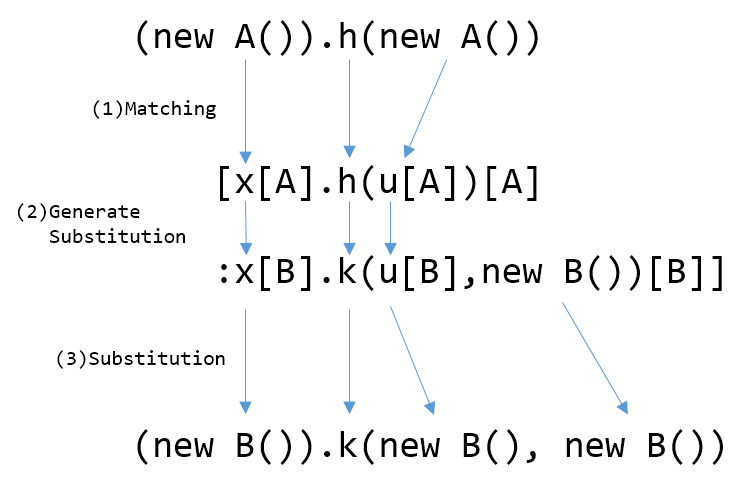
\includegraphics[width=6cm]{example1.png}
%    \caption{An example}
%    \label{exofuc}
%\end{figure}
%\par
%Other evaluation rules are similar to the rule E-INVOKE. And in some cases, a Java term may not be matched by any of the rules and we have E-ALTER-NEW and E-ALTER-INVOKE to transform the code. For E-CLASS, we can easily translate a class name in old API to a class name in new API if there is a type mapping specified in the SWIN body $\tt \Pi$.


%%% Local Variables: 
%%% mode: latex
%%% TeX-master: "pepm-15"
%%% End: 


\begin{section}{Type Checking System for Core SWIN}
\label{tw-type}

Now we turn to our type system that is used to check the type safety
of transformation programs in SWIN. Given two APIs, $\tt API_s$ and
$\tt API_d$, and a transformation program, $\tt\Pi$, mapping from $\tt
API_s$ to $\tt API_d$, if $\tt\Pi$ passes our type checking, we can
guarantee that $\tt\Pi$ will transform {\em any} FJ program using $\tt
API_s$ to a well typed FJ program using $\tt API_d$ instead. % $\tt
% API_s$ and $\tt API_d$ are used to refer to the source API and target
% API respectively (the formal definition of $\tt API$ can be referred
% to \ref{APIdef}).

% \begin{figure}
% \begin{align*}
%  \tt API ~ ::=&\tt ~ \{ ~ \overline{CL} ~ \}       & \text{API definition}\\
%  \tt E ~   ::=&\tt ~ \{~ \overline{x:C_1\hookrightarrow C_2}~\}     & \text{SWIN environment}
% \end{align*}
% \caption{Auxiliary Definition. $\tt API$ is defined as a set of class declarations, and an $\tt API$ itself is a well typed FJ program. $\tt E$ is the type checking environment, which contains the type migration information of variables appeared in rules.}
% \label{APIdef}
% \end{figure}

% In the
% case of API update, $\tt
% API_s$ should include only the changed part, i.e.,
% $\tt API_s$ contains only these 
%
%To claim that a piece of update code $\tt\Pi$ that transform client
%codes with a source API ($\tt API_o$) to an new API ($\tt API_n$) is
%type-safe, we need to have this update code $\tt\Pi$ can transform any
%well typed client source code with $\tt API_o$ to a new one that is
%also well typed under FJ type system.
%
%\par
%To keep the safe property mentioned above, we give restrictions on the update language and check whether a piece of update code conserves the relationship between the old API and the target API. We present a type system for SWIN language to check both the SWIN grammar and the safety conditions mentioned in Section \ref{sec:examples}.
%\par
In the following sections, we will define our type-checking rules and 
prove the type-safety property of SWIN.

\begin{figure}[htb!]
% \begin{center}
% \AXC{$\tt
%   x:C_1\hookrightarrow C'_1,~\bar{y}:\overline{C_2\hookrightarrow C'_2}~ \in
%   E$}
% \AXC{$\tt class\ C_1\ extends\ D \{\bar{C}\ \bar{f}; K\ \bar{M}\}\in API_s$ ~~~~ $\tt C_d\ m(\bar{C}_s\ \bar{u})\{...\} \in \bar{M}$}
% \AXC{$\tt \bar{C}_2<:\bar{C}_s$}                                            \RightLabel{~(T-L1)}
% \TIC{$\tt E\vdash_l x.m(\bar{y}):C_d$}
% \DP
% \end{center}
% \vspace{2pt}

% \begin{center}
% \AXC{$\tt class\ C\ \{\ \bar{C}\ \bar{f}; C(~\bar{C}_s\ \bar{u}~) \{...\}\ \bar{M}\}\in API_s$}
% \AXC{$\tt
%   \bar{x}:\overline{C_1\hookrightarrow C'_1} \in E$}
% \AXC{$\tt \bar{C}_1<:\bar{C}_s$}                                    \RightLabel{~(T-L2)}
% \TIC{$\tt E\vdash_l new\ C(\bar{x}):C$}
% \DP
% \end{center}
% \vspace{2pt}

% \begin{center}
% \AXC{$\tt
%   E=\{\bar{x}:\overline{C\hookrightarrow D}\}$}
% \AXC{$\tt \{~\bar{x}:\bar{D}~\}\vdash_{FJ}^{API_d} t:C_d$}
% \RightLabel{~(T-R)}
% \BIC{$\tt E\vdash_r t:C_d$}
% \AXC{$\tt \{~\bar{x}:\overline{C\hookrightarrow D}~\}\vdash_l l:C_1,\
%   \{~\bar{x}:\overline{C\hookrightarrow D}~\}\vdash_r r:C_2$}             
% \RightLabel{~(T-$\pi$)}
% \UIC{$\tt [\{~\bar{x}:\overline{C\hookrightarrow D}~\}\ l:C_1\rightarrow r:C_2]~\mathit{ok}$}
% \noLine
% \BIC{}
% \DP
% \end{center}

\begin{center}
  \AXC{$\tt \{~\bar{x}:\bar{C}~\}\vdash_{FJ}^{API_s} l:C_1$}
  \AXC{$\tt \{~\bar{x}:\bar{D}~\}\vdash_{FJ}^{API_d} r:C_2$}
\RightLabel{~(T-$\pi$)}
\BIC{$\tt [\{~\bar{x}:\overline{C\hookrightarrow D}~\}\ l:C_1\rightarrow r:C_2]~\mathit{ok}$}
\DP
\end{center}
\vspace{2pt}
\caption{Checking rule for $\pi$}
\label{typerules}
\end{figure}

\newcommand{\indentspace}{~~~~~~~~}

\begin{figure*}
\begin{align*}
% Curr
%\tt \mathbf{ClassCover}&\tt(\Pi, API_s, API_d) =\\
%                  &\tt \forall~C_1. (class\ C_1\ extends\ \_~\{ ... \}\in (API_s-API_d) \\
%                  &\tt \indentspace\Rightarrow~ \exists~C_2.(class\ C_2\ extends\ \_\in API_d \land C_1\hookrightarrow C_2\in \mathbf{TypeMapping}(\Pi)))\\
\tt \mathbf{RuleOK} &\tt(\Pi) = \forall~\pi. (\pi\in\Pi \Longrightarrow \pi~\mathit{ok})\\
\tt \mathbf{ConstrCover}&\tt(\Pi, API_s, API_d) =\\
                  &\tt \forall~C_1,\bar{C}. (class\ C_1\ extends\ \_~\{ C_1(\bar{C}\ \bar{\_})~...~\}\in (API_s-API_d) \\
                  &\tt \indentspace\Rightarrow~ \exists~C_2,\bar{C}',\bar{x},r.((~\bar{x}:\overline{C\hookrightarrow C'}~)[new\ C_1(\bar{x}):C_1\rightarrow r:C_2]\in\Pi))\\
\tt \mathbf{MethCover}&\tt(\Pi, API_s, API_d) =\\ 
                  &\tt \forall~C_1,C_2,m,\bar{C}.(class\ C_1\ extends\ \_~\{~C_2\ m(~\bar{C}\ \bar{\_}~)\{...\}~...~\}\in (API_s-API_d) \\
                  &\tt \indentspace\Rightarrow~ \exists~x,\bar{y},C'_1,C'_2,\bar{C}',r.((x:C_1\hookrightarrow C'_1,\ ~\bar{y}:\overline{C\hookrightarrow C'}~)[x.m(\bar{y}):C_2\rightarrow r:C'_2] \in \Pi))\\
\tt \mathbf{FieldCover}&\tt(\Pi, API_s, API_d) =\\ 
                  &\tt \forall~C_1,C_2,f.(class\ C_1\ extends\ \_~\{C\ f;...\}\in (API_s-API_d) \\
                  &\tt \indentspace \Rightarrow~ \exists~x,C'_1,C'_2.((x:C_1\hookrightarrow C'_1~)[x.f:C_2\rightarrow r:C'_2] \in \Pi))                           \\
\tt \mathbf{MapChecking}&\tt(\Pi, API_s, API_d) =\\
                  &\tt \forall~C,D.(C\hookrightarrow D\in \mathbf{TypeMapping}(\Pi)\\
                  &\tt \indentspace\Rightarrow~ (\exists~CL\in API_s \cap API_d. (\mathbf{Decl}(CL)=C \land D = C))\\
                  &\tt \indentspace\indentspace \lor (\exists~CL\in API_s-API_d. (\mathbf{Decl}(CL)=C)))\\
\tt \mathbf{Subtyping}&\tt(\Pi, API_s, API_d) = \\
                      &\tt\forall~C_i,D_i,C_j,D_j.( C_i\hookrightarrow D_i, C_j\hookrightarrow D_j \in \mathbf{TypeMapping}(\Pi) ~~\Rightarrow~~ (C_i <: C_j\Rightarrow D_i<:D_j))\\
\tt \mathbf{TypeSafe} &\tt(\Pi, API_s, API_d) = \\
                      &\tt \mathbf{RuleOK}(\Pi) \land \mathbf{ConstrCover}(\Pi, API_s, API_d) \land \mathbf{MethCover}(\Pi, API_s, API_d)\\
                      &\tt \land \mathbf{FieldCover}(\Pi, API_s, API_d) \land \mathbf{MapChecking}(\Pi, API_s, API_d) \land \mathbf{Subtyping}(\Pi, API_s, API_d)
\end{align*}
\caption{Checking rules for $\tt\Pi$. A SWIN program ($\tt\Pi$) with specified source API ($\tt API_s$) and destination API ($\tt API_d$) should pass these checking rules to maintain type safety. Underscore(\_) is a wildcard and apostrophe (...) represents omitted declaration sequences (field declarations or method declarations). }
\label{logicrules}
\end{figure*}

\begin{subsection}{Type Checking Rules}

  We present the rules in Figure~\ref{typerules} and
  Figure~\ref{logicrules}. Figure~\ref{typerules} depicts the rule
  for checking a single transformation rule $\pi$.
  Figure~\ref{logicrules} depicts the rules for checking a
  transformation program $\Pi$.

  \paragraph{Checking Rule for $\pi$} This rule checks whether the
  types declared in a transformation rule conforms to the actual types
  inferred using FJ typing rules. In the formal notation, we use
  $\tt\Gamma\vdash^{API_s}_{FJ}t:C$ to denote that the term $\tt t$ has type $\tt C$
  under context $\tt\Gamma$ by FJ typing rules when considered together with
  $\tt API_s$.

  Please note that this rule also indicates that we can drop the type
  declarations in the transformation rules, i.e., instead of
  writing $\tt [\ x.m(y):C \rightarrow x.h(y):D\ ]$, we can write $\tt[\
  x.m(y) \rightarrow x.h(y)\ ]$ and deduce $\tt C$ and $\tt D$ using FJ typing
  rules. However, we find that with the return type explicitly declared in the code,
  we could make $\tt \mathbf{TypeMapping}(\Pi)$ explicit, avoiding subtle bugs
  on erroneous type mappings. As a result, we require the user to
  declare types of the transformed terms. 

%   \paragraph{}
  
  
% Figure \ref{typerules} gives the detailed definition of the SWIN type
% checking rules. The goal is to check the rule against {$\tt \mathbf{TypeSafe}$} for a SWIN program $\tt \Pi$. 
% Given two APIs ($\tt API_s$ and $\tt API_d$) and a SWIN program $\tt \Pi$, the checking rule $\tt \mathbf{TypeSafe}$ will check type safe property of the SWIN program in the following aspects:

% \begin{itemize}
% \item Each rule is well formed.  ($\mathbf{RuleOK}$)
% \item For each class constructor, method or field in a class belongs to $\tt API_s-API_d$, there are corresponding rules to transform their usage. ($\mathbf{ConstrCover}, \mathbf{MapChecking}$ and $\mathbf{FieldCover}$)
% \item Subtyping relationship will be preserved through transformation process, and the mapping between source API type and target API type should be a function. ($\mathbf{Subtyping}$)
% \item The SWIN program will not migrate a class in $\tt API_s\cap API_d$. ($\mathbf{MapChecking}$)
% \end{itemize}

% \paragraph{Notations}

% %For each transformation rule, we check its source code pattern (T-L1, T-L2),
% %destination code pattern (T-R). If both of its code pattern is well formed, the transformation rule $\pi$ is well typed.

% % In the definition, we use \todo{thename} to look up
% % the type of a method. Please note that in FJ there is no method
% % overloading, so it is enough to specify only the method name and the
% % class name.

% In the checking rules, $\tt E\vdash_{l} \mathit{l}$ represents the type inference for left hand side code pattern ($\mathit{l}$) under SWIN typing context $\tt E$ and $\tt E\vdash_{r} \mathit{r}$ represents the type inference on the right hand side code pattern. The definition of SWIN typing context $\tt E$ can be referred to \ref{APIdef}, which is the typing context for variables appeared in SWIN programs.

% Besides, we use $\tt \{\bar{x}:\bar{D}\}\vdash^{API}_{FJ} t:C_d$ to denote that a FJ term has type $\tt C_d$ under FJ typing system and . And $\tt API_s-API_d$ is use to represent the set complements on $\tt API_s$ and $\tt API_d$. 

% We use judgment $\tt E\vdash \bar{e}:\bar{T}$ to denote 
% that under typing environment $\tt E$ (which describes
% mapping from meta variables to their types), $\tt \bar{e}$ has
% type $\tt \bar{T}$. It checks variables (by T-VAR), source code patterns 
% (by T-L1, T-L2), target code patterns (by T-R),
% update rules (by T-$\pi$), and the whole update program (by T-$\Pi$).
% Note that in rule T-R, we use $\tt \{API_d,\bar{x}:\bar{D}\}\vdash_{FJ} t:C_d$,
% a type check judgment provided by FJ, to check whether 
% an FJ term $\tt t$ is type-corrected.

% With these rules, an update program $\tt\Pi$ is typed to
% $\tt\{\overline{C\rightsquigarrow D}\}$ if it passes the following two checks.
% %
% First, it checks whether variables in an update rule $\tt\pi$ are
% bounded in the variable declaration part of $\tt \pi$. This is done 
% in rules T-L1, T-L2 and T-R.
% %
% Second, it checks whether update program $\tt \Pi$ satisfies the four
% conditions mentioned in Section 2.

\paragraph{Checking rules for $\tt\Pi$}
The main goal of the type checking rules is to check the four
conditions presented in Section~2. Next we explain how this is achieved.

\todo{Chenglong, can you make the following description consistent
  with your new definition?}

\begin{enumerate}
\item For each rule $\tt\pi$, let the variable declaration be
  $\tt\bar{x}:\overline{A\hookrightarrow B}$. Then source code pattern $\tt
  l$ is well typed under the variable environment
  $\tt\Gamma_s=\{\bar{x}:\bar{A}\}$ and target code pattern is well
  typed under $\tt\Gamma_d=\{\bar{x}:\bar{B}\}$. (Rules T-L1,T-L2 and
  T-R guarantee this property.)

\item The class mapping in $\tt \mathbf{TypeMapping}(\Pi)$ should be a
  function, i.e. one class in the old API should be mapped to only one
  class in new API. In fact, this property is covered by the subtyping relationship check,
  as type equality can be treated as a bi-direction subtyping
  relation. (Rule $\mathbf{Subtyping}$ guarantees this property.)

\item The class transformation preserves the subtyping relationship in the old
  API. (Rule $\mathbf{Subtyping}$ guarantees this property)

\item The transformation program covers all classes/methods/constructors/fields only
  in the old API (Rules \textbf{ConstrCover}, \textbf{MethCover}, \textbf{FieldCover}), as well as all type changes required in the type
  mapping (Rule $\mathbf{MapChecking}$). 
  The property of the ``class cover'' (i.e. there should be a corresponding rule to transform each class appeared in $\tt API_s-API_d$) 
  can be achieved by rule $\mathbf{ConstrCover}$ and the definition of $\mathbf{TypeMapping}$. 
\end{enumerate}

As will be proved in Section \ref{sec:theorem}, if the above checks
succeed, a transformation program $\tt\Pi$ will be type-safe, guaranteeing the
well-typedness of the target code when $\tt\Pi$ is applied to any
client code with old API. Otherwise, there must exist some client code
that cannot be transformed to a well typed target code with this
transformation program.

% \todo{Hu revised Section 4 till here. Please check my revision,
% and improve the rest of this section. If we do not have much space,
% the example below may be removed.}

% Again, we take the example in section 2 to explain the type checking
% procedure. Suppose we use SWIN to update client code using $\tt API_1$
% (a subset of SWING) to client codes with $\tt API_2$ (a subset of SWT). Namely,
% \begin{align*}
% \tt API_1=\{\tt &\\
% 			 &\tt class\ JFrame\ extends\ Container\\
% 			 &\qquad\tt\{new\ JFrame()\{...\}\},\\
% 			 &\tt class\ JList\ extends\ Container\\
% 			 &\tt\qquad\{new\ JList()\{...\}\},\\ 
% 			 &\tt class\ Container \\
% 			 &\qquad\tt\{new\ Container()\{...\}\}\\
% 			\}\\
% %\end{align*}
% %\begin{align*}
% \tt API_2=\{ &\tt\\
% 			 &\tt class\ Shell\ extends\ Composite\ \{new\ Shell()\{...\}\},\\
% 			 &\tt class\ List\ \tt\{new\ List()\{...\}\},\\
% 			 &\tt class\ Composite\ \\ 
% 			 &\qquad\tt\{new\ Composite(Shell\ x, Integer\ y)\{...\}\}\\
% 			\}
% \end{align*}
% As in Figure~\ref{fig-swingtoswt}. Subtyping in $\tt API_1$ is
% \begin{align*}
% \tt JFrame <: Container \\
% \tt JList <: Container
% \end{align*}
% And there is only one subtypeing relation is $\tt API_2$:
% \begin{align*}
% \tt Shell <: Composite 
% \end{align*}
% We have the following SWIN code to update the old client code:
% \begin{align*}
% \tt \Pi=&\tt 	\{\pi_1,\pi_2,\pi_3\}\\
% {\bf where}\\
% \tt \pi_1=&\tt 	()[new\ Container():Container \\
% 			&\tt\rightarrow new\ Composite(new\ Shell(), 0):Composite]\\
% \tt \pi_2=&\tt 	()[new\ JList():JList\rightarrow new\ List():List]\\
% \tt \pi_3=&\tt 	()[new JFrame():JFrame\rightarrow new\ Shell():Shell]
% \end{align*}

% For the rule $\pi_1$, its source code pattern $\tt new\ Container():Container$ can be typed to $\tt Container$ by type checking rule T-L1, and target code pattern $\tt new\ Composite(new\ Shell(), 0):Composite$ can be typed to $\tt Composite$ by type checking rule T-R and thus they pass the checking rule 1 (Grammar checking). Then according to the rule T-$\pi$, there is no unbounded variables thus $\tt\pi_1$ is well typed and it has type $\tt Container\rightsquigarrow Composite$. Similarly, $\pi_2$ and $\pi_3$ are well typed, $\tt\pi_2:JList\rightsquigarrow List$ and $\tt \pi_3:JFrame\rightsquigarrow Shell$.
% \par
% Then the final step of type inference is to infer the type of $\tt\Pi$. According to the rule T-$\Pi$, $\Pi=\{\pi_1,\pi_2,\pi_3\}$ holds the property:
% \begin{enumerate}
% \item $\tt\Pi$ covers all the APIs defined in $\tt API_1$.
% \item $\tt\Pi$ is a function on classes in $\tt API_1$.
% \end{enumerate}
% But $\Pi$ in this case does not preserve the subtyping relation as $\tt JList <: Container$ in old API but $\tt \Pi(JList)=List \nless: Composite=\Pi(Container)$. Thus $\Pi$ is not well typed under SWIN type system, thus this SWIN code is not safety. 
% \par
% And if we have a function defined in client code: $$\tt class\ A\ \{void\ f(Container C){...}\}$$ 
% It is clear that the following code:
% $$\tt new\ A().f(new JList())$$
% is well typed with old API. But after update, it is not well typed as $\tt new\ A().f(new List())$ will meet an argument type error for the updated function definition $\tt A\ \{void\ f(Composite C){...}\} $. (As subtyping relation is not preserved in new API).
% \par
% On the other hand, if SWIN code is well typed (thus passing grammar checking and safety checking), we have the theorem in the next subsection to guarantee that it will safely update any client code using the old API.

\end{subsection}

\begin{subsection}{Type-Safety Theorem}
\label{sec:theorem}

In this subsection, we present the type-safety property of a well-typed SWIN program formally and outline the key theorems and lemmas here. 

Intuitively, the type-safety property of a well-type SWIN program is that a well-typed SWIN program can transform \emph{any} FJ program to a well typed FJ program. The the proof needs to bridge the type inference tree on an old
API to the new type inference tree on a new API, and we need to generate
a derivation tree based on conditions in checking rules and the
derivation tree on original client code.

Because of the space limit, we cannot present the full proof
here. Instead, we present five key lemmas that can stepwise lead to
the final theorem. The full proof of lemmas and the theorem
can be found in  the technical report on the formal definition of SWIN. \todo{cite the TR}
% language~\cite{proof}.

In our lemmas, $\tt\Gamma=\bar{x}:\bar{C}$ represents the typing context of a FJ term $\tt t$, which designates each variable $\tt x$ in the term with a type $\tt C$.  Specially, given a term $\tt t$ in client code and a transformation program $\tt\Pi$, $\tt\Gamma_s$ represents the variable environment for $\tt t$ (before transformation) and $\tt\Gamma_d$ represents the environment of the transformed term $\tt\Pi(t)$.
%\end{def1}

% Specially, in our lemmas, we use $\tt\Gamma_s$ to denote the variable environment for client code with old API, and $\tt \Gamma_d$ to denote the variable environment for client code with new API. 

\begin{lemma}[Typing Context]
Given a SWIN program $\tt\Pi$ acting on $\tt API_s$ to $\tt API_d$, suppose the typing context for a term $\tt t$ is $\tt\Gamma_s = \bar{x}:\bar{C}$ , then the typing context for $\tt\Pi(t)$ is $\tt\Gamma_d=\bar{x}:\overline{\Pi(C)}$.
\end{lemma}
\begin{proof}
Note that FJ typing context $\tt\Gamma$ will be created in the rule FJ-M-OK and will not change during type derivation of a term. According to the rule E-DELCARATION and E-METHOD, both the method argument types and the class type will be updated to $\tt\Pi(C)$.
\end{proof}
%\todo{do you want to present a lemma or a definition in Lemma 1? If a lemma,
%  what are the definitions of $\Gamma_s$ and $\Gamma_d$? If a
%  definition, change it to a definition.}

\begin{lemma}[Subtyping]
Suppose $\tt \Pi$ passes SWIN type checking rules, and it transforms an FJ program with $\tt API_s$ to a new program with $\tt API_d$, then:\par
$\tt C_1<: C_2 $ in old program ~~$\Longrightarrow$~~ $\tt\Pi(C_1)<:\Pi(C_2)$ in the transformed program.
\end{lemma}
\begin{proof}
The subtyping relationship between classes have the following two cases:
\begin{itemize}
\item $\tt C_1$ is declared in client code: E-DECLARATION will guarantee that subtype relationship will be preserved in transformation.
\item $\tt C_1$ is declared in API: the checking rule $\mathbf{Subtyping}$ guarantees it. 
\end{itemize}
Combining these two cases and the transitional subtype relationship, the subtyping relationship will be guaranteed.
\end{proof}

\begin{lemma}[Variable Substitution]
Suppose that an FJ term $\tt t$ is well typed under context $\tt \Gamma=\Gamma_1,\{\bar{x}:\bar{C}_x\}$, i.e. $\tt \Gamma\vdash_{FJ} t:C_t$, then after substituting terms $\tt \bar{t}_v$ for variables $\tt \bar{x}$ , with the property that $\tt\Gamma_1\vdash_{FJ}\bar{t}_v:\bar{C}_v$ and $\tt\bar{C}_v <: \bar{C}_x$, $\tt t$ can be typed to $\tt C_t$ or a sub-class of $\tt C_t$. Namely,
$$\tt \Gamma_1,\{\bar{x}:\bar{C}_x\} \vdash_{FJ} t:C_t \Longrightarrow \Gamma_1\vdash_{FJ} [\bar{x}\rightarrow\bar{t}_u]t: C'_t,\ C'_t <: C_t$$
\end{lemma}
\begin{proof}
By induction on the derivation of a term $\tt t$, we have fives cases to discuss. ($\tt x$, $\tt(C)t$, $\tt t.f$, $\tt new~C(\bar{t})$ and $\tt t.m(\bar{t})$).
The first three cases ($\tt x$,$\tt (C)t$ and $\tt t.f$) are obvious according to their evaluation rules.

For case 4 and case 5, the following properties are used in proof:
\begin{itemize}
\item The arguments in the method invocation will be substitute by terms whose types are subtypes of the original argument variables (Arguments are compatible).
\item The target term (the caller) is of a type that is subtype to the original caller variable (The method can be found in the new caller term).
\end{itemize}
With these subtyping relation cleared, the proof is also obvious according to the rule FJ-METHOD and FJ-CONSTRUCTOR.
\end{proof}

\begin{lemma}[Term Formation]
Suppose we have a well typed SWIN program $\tt \Pi$, if a term $\tt t$ in the original typing context can be typed to $\tt C$, then after transformation, the term is well typed and its type is a subtype of $\tt \Pi(C)$. i.e.
$$\tt \Gamma_s\vdash^{API_s}_{FJ} t:C \Longrightarrow \Gamma_d\vdash^{API_d}_{FJ} \Pi(t):C',\ where\ C'<:\Pi(C)$$
\end{lemma}
\begin{proof}
By induction on the term derivation. Again we have five cases to prove. ($\tt x$, $\tt(C)t$, $\tt t.f$, $\tt new~C(\bar{t})$ and $\tt t.m(\bar{t})$)

The first two cases ($\tt x$, $\tt (C) t$) are obvious according to Lemma 1 and their evaluation rules.
The last three cases are not trivial in proof, we simply mention some points for case 5 (method invocation) as an example, and the proof can be referred to TR \todo{cite TR}.

For case $t=t_0.m(\bar{t}_u)$, we have two subcases to deal with:
\begin{itemize}
\item The method is defined in a class which is defined in client code: to prove that arguments and the caller terms are well formed terms whose types are subtypes of the original ones.
\item The method is defined in a class defined in old API: to prove that the rule $\tt\pi$ to transform the term will finally leads to a well-typed term according to the Substitution Lemma and Subtyping Lemma.
\end{itemize}

And with these five cases proved, we have a well type SWIN program can correctly transform FJ terms.
\end{proof}

\begin{theorem}[Type-Safety]
Class declarations are well typed after a transformation by a well typed SWIN program $\tt \Pi$. 
i.e. For any \verb|CL|,
 $$\tt \Pi(CL)= class\ \Pi(C_1)\ extends\ \Pi(C_2)\ \{\ \Pi(\bar{C}_i)\ \bar{f}_i;\ \Pi(K)\  \overline{\Pi(M)}\ \}$$
is well typed with new API if $\tt \Pi$ is well typed.
\end{theorem}
\begin{proof}
We need to prove that method calls are well formed in the transformed FJ program and the class declarations are well formed.

This can be obvious as all terms are well formed after transforamtion (Lemma 4), and according to the evaluation rules E-METHOD-DECLARATION and E-CLASS-DECLARATION, the fact that all declarations are well formed can be easily proved by going through declaration details.
\end{proof}

With the type-safety theorem proved, a well typed SWIN program can transform any FJ client code safely.
\end{subsection}

\end{section}






%%% Local Variables: 
%%% mode: latex
%%% TeX-master: "pepm-15"
%%% End: 


\begin{section}{From Core SWIN to Full SWIN% Extending to Full Java
  }
\label{sec:extension}

In this section, we present the way to extend core SWIN on
Featherweight Java to full SWIN on full Java language formally.
Generally, the extension is based on the term extension and type
extension. By extending source code pattern and target code pattern to
a term in full Java and extending types to full Java in variable
declaration part of update rules, we are able to match a Java term and
then transform it to a term with new API by meta-variable
substitution.
\par
Extending SWIN to full SWIN, we need some special treatments of the following key points :

\paragraph{Package} % In full Java, $\tt import$ command allows us to
                    % import a package at the head of a program and
                    % use classes in the package without using the
                    % full name. In this case, when we update APIs in
                    % the package, we will match the short name if it
                    % is not ambiguous and transform it to a short
                    % name in target API, and then generate a $\tt
                    % import$ command in the head of target client
                    % code.
Full Java supports the \code{package} and \code{import} commands for name organization. To ease the writing
of transformation rules, we also support \code{import} command in
SWIN, yet all internal processing is based on fully qualified names.

%<<<<<<< .mine
%\paragraph{Assignment} 
%When we extend SWIN to full Java with assignment, we need to consider the problem with side effect.
%To keep the update process still holding type safety, we need to distinguish the difference the application of $\tt\Pi$ on a L-value between that on a R-value.
%We need to check that an update rule will not transform a L-value to a R-value. And when we apply SWIN on an assignment expression, we simply apply it on both sides. 
%=======
\paragraph{Field and Assignment} 
%When we extend SWIN to full Java with assignment, we need to consider
%the problem with side effect.
FJ has no assignment statements and all fields are read-only. When assignments are introduced, expressions in Java can be
distinguished into L-value and R-value. To ensure type safety, we need
to ensure the transformation does not change an L-value into an
R-value. The most common L-value is field access. For example, given ``\code{a.x = b}'', if a transformation rule
transforms ``\code{a.x}'' into ``\code{new A()}'', the new code will fail to
compile because ``\code{new A()}'' is not a L-value. This check can be
implemented by applying the Java rules for distinguishing L-value and
R-value on the source patterns and the destination patterns.
%>>>>>>> .r506

% To keep the update process still holding safety property, we need to distinguish the difference the application of $\tt\Pi$ on a L-value between that on a R-value.
% We need to check that an update rule will not transform a L-value to a R-value. And when we apply SWIN on an assignment expression, we simply apply it on both sides. 

\paragraph{Static Method Access} In full Java, a method can be defined
as a static method, and we can access it by $\tt C.m(a,b,...)$. 
We treat the application of full SWIN on static method access as a normal method invoke, except that we 
need to apply the term directly on the class identifier. As the transformation of a class definition is 
by class name replacement, type safety can be guaranteed.

\paragraph{Overload} % Method overloading in full Java may lead to problems in the matching process.
% As we allow a meta-variable $\tt x$ of type $\tt A$ in source code
% pattern matches a term $\tt t$ with a subtype of $\tt A$, this may
% lead a piece of client code match more than one update rules. And this
% ambiguity can be resolved if we define a matching order on a FJ term
% with subtyping relation: we will always choose one with closest
% subtyping relation to match the term.  For
% example, if we have a relationship $\tt A<:B<:C$, and in class $\tt
% D$, we have methods $\tt f(B\ x)$ and $\tt f(C\ x)$. Then $\tt(new\ D()).f(new\
% A())$ will be matched to the first pattern as they have a closer
% subtyping relationship.
When method overloading is considered, we need to match a method not
only using its name, but also the type of its input parameters. Also,
the subtyping relation should be considered in the same way as Java:
when there are several overloaded methods that can be matched, we
choose the one with the closest subtyping relation on the parameters. For
example, if we have a relationship $\tt A<:B<:C$, and in class $\tt
D$, we have methods $\tt f(B\ x)$ and $\tt f(C\ x)$. Then $\tt(new\ D()).f(new\
A())$ is a call to the first method as they have a closer
subtyping relationship. A pattern matching $\tt f(C\ x)$ should not match
this term.

\paragraph{Generics} Generics in full Java affects the evaluation rules E-CLASS
and E-T-NEW. We have two extending rules to solve this problem.
\begin{enumerate}
    \item During pattern matching, a rule matches a generic type without considering
        parameterized types.
    \item After performing transformation on the generic type, 
        our rules recursively visit the parameterized types.
\end{enumerate}
% These two rules can assure the well-typedness of a term with parameterized types during transformation.
% The limitation of this way is that the generic class should not changes the number of
% type parameters during evolution which is reasonable in real APIs evolution.
The type safety is guaranteed because we require the preservation of
subtyping relation, and thus the constraints on generic parameters
will not be broken. The limitation of this method is that the number
of type parameters in a generic class cannot change from the source
API to the target API. However, we have never observe this kind of
change in practice.
\end{section}


%%% Local Variables: 
%%% mode: latex
%%% TeX-master: "pepm-15"
%%% End: 


\section{Case Studies}
\label{sec:evaluation}
\subsection{Research Questions}
Since SWIN puts two more conditions on the replacement rules than
Twinning, a natural question to ask is whether these two additional
conditions confine the expressiveness of the language. In other words,
there are programs that can be written in Twinning but not in SWIN,
but are these programs useful in practice? Furthermore, beyond
Twinning, we also want to understand the expressiveness of SWIN in
general. These considerations lead to two research questions.
\begin{enumerate}
\item Does the extra conditions confine the expressiveness of SWIN
  compared with Twinning? %How much expressive is SWIN compared with Twinning?
\item In general, how much expressive is SWIN?
\end{enumerate}

\subsection{Study Setup}
To answer the two research questions, we perform three case
studies. To answer the first research question, we need to compare
SWIN with Twinning. To do this, we repeat a case study in Twinning
that migrate programs from Crimson v1.1.3\footnote{\url{http://xml.apache.org/crimson/}}
to dom4j v1.6.1\footnote{\url{http://www.dom4j.org/}}. Crimson and
dom4j are both Java libraries for manipulating XML files, but Crimson
is no longer supported. Thus, developers may want to migrate programs
from Crimson to dom4j.

To answer the second research question, we further perform two more
case studies, one is about migration from one API to another API, the
other one is to upgrade clients for incompatible API upgrade. More
concretely, we chose the program migration from Twitter4J v4.0.1\footnote{\url{https://github.com/yusuke/twitter4j/}}
to
Sina Weibo Java API v2\footnote{\url{https://code.google.com/p/weibo4j/}}, 
and the client upgrade from Google Calendar
API\footnote{\url{https://developers.google.com/google-apps/calendar/}}
v2 to v3. Twitter4J is a Java wrapper for the RESTful Twitter
API. Sina Weibo is the Chinese counterpart of Twitter, and it provides
an official Java library for accessing its web API. Google Calendar
API is the official Java library for accessing the data in Google
Calendar.

The two case studies of program migration (from Crimson to dom4j, from
Twitter4J to Sina Weibo API) both involve large APIs, and it is
difficult for us to cover the full APIs. In the case study from
Crimson to dom4j, the Twinning authors~\cite{twinning} chose a client
(log4j v1.2.14\footnote{\url{http://logging.apache.org/log4j/1.2/}}) 
and only wrote transformations for the part of the API
covered by the client. We followed the same step as their case
study. In the case study from Twitter4J to Sina Weibo API, we consider
three example clients on manipulating the timeline provided in the example
directory in the Twitter4J source package, and cover only the part of
the API used in these examples.

To perform the case studies, we implemented SWIN in Java using
the Polyglot compiler framework~\cite{glot}. Both our
implementation and all evaluation data are available at the project
web site\footnote{\url{https://github.com/Mestway/SWIN-Project}}.

\subsection{Results}\label{sec:results}


\subsubsection{General Expressiveness}
In total, we wrote 94 rules for the three case studies, each
transforming a method call to the old API into an expression using the
new API. Our rules cover 97\% of the total API methods that needed to
be transformed in the three case studies. This results indicate that,
though our approach deals only with one-to-many mappings, it is able
to perform a significant portion of program adaptation tasks in
practice.

\subsubsection{Comparison with Twinning}
The only uncovered API changes are three method changes in
Google Calendar API, consisting of 3\% of the total API methods that
needs to be transformed. In the three uncovered method changes, one
method splits into several methods, and we need to decide which
new method to replace the original one based on the calling context,
which is not supported in SWIN.

More concretely, method ``\code{EventWho.getAttendeeType()}'' in
Google Calendar v2 returns a string that may contain either
``attendee'' or ``organizer''. Google Calender v3 replaces this method
with two methods: ``\code{boolean getSelf()}'' which returns true when
 ``attendee'' should be returned and ``\code{boolean getOrganizer()}'' which
returns true when ``organizer'' should be returned. To migrate the
client, we may need to transform the code as follows, where
``\code{getSelf()}'' is a client-written method to test whether the
argument is equal to ``attendee'',
\begin{lstlisting}
String attendeeType = attendee.getAttendeeType();
boolean isSelf = isAttendee(attendeeType);  
\end{lstlisting}
into the code as follows.
\begin{lstlisting}
boolean isSelf = attendee.getSelf();  
\end{lstlisting}

This example shows two fundamental limitations of SWIN. First, to
perform the above transformation, we need to match a sequence of
statements and transform them into one method calls. This requires
many-to-one mapping and is not supported by SWIN. Second, we need to
perform a semantic analysis on the implementation code of
\code{isAttendee} to decide whether to transform the code into
\code{getSelf()} or \code{getOrganizer()}. This kind of conditional
transformation is not supported by SWIN.

Clearly, Twinning also has these limitations and cannot handle the
three split methods in Google Calendar API as well. This result
indicates that SWIN is as expressive as Twinning on our three case
studies. Please note that many API classes have sub classes, and thus
the SWIN programs should be much shorter than Twinning, as in Twinning
we need to repeat the rules for the parent class also on each sub
class. % The result also indicates that SWIN is expressive in general,
% being able to handle the transformation of the majority (97\%) of the
% methods in our case studies.

\subsubsection{Interesting Transformation Patterns}
In the implementation of the three case studies, we also found that
many transformations are not direct method replacement, but can still
be expressed in SWIN by flexible use of the transformation rules. We
summarize three patterns below.

\smalltitle{Method $\leftrightarrow$ Constructor} We may need to
map between class constructors and methods, and in SWIN we can
directly specify such a replacement. For example, in the case from
Crimson to dom4j, we write the following piece of code. This program
is in the text form of SWIN, where we use \texttt{->>} to denote $\hookrightarrow$
and \texttt{->} to denote $\rightarrow$.
\begin{lstlisting}
(f : DocumentBuilderFactory ->> DocumentFactory)
[ (f.newDocumentBuilder()):DocumentBuilder ->
    (new SAXReader(f)):SAXReader ]
\end{lstlisting}

\smalltitle{Type Merging} Sometimes a set of classes in the old API
become one class in the new API. In class \texttt{CalendarEvent} in
Google Calendar v2, there is a method \texttt{getTitle()}. Developers
can use this method to acquire the title of a source, but the type of
the title is \texttt{TextConstruct}.  Class \texttt{TextConstruct} is
a wrapper of a string, and there is a method \texttt{getPlainText()}
which returns the internal string. In Google Calendar v3, the class
\texttt{CalendarEvent} becomes \code{Event}, which directly contains a
method \code{getSummary()} to return the string of title. As a result,
we may need to transform a sequence of method invocations
``\code{x.getTitle().getPlainText()}'' into a single invocation ``\code{x.getSummary()}''.

Although such a transformation implies a many-to-many mapping%  seems similar to the many-to-one
% mapping mentioned above
, it can be implemented in SWIN because
\code{TextConstruct} is only used in the return type of
\code{getTitle()} in Google Calendar API. We can consider the API
upgrade as merging classes \code{CalendarEvent} and \code{TextConstruct} into
\code{Event} and merging methods \code{getTitle()} and
\code{getPlainText()} into \code{getSummary()}. As a result, we can
remove the call to \code{getPlainText()} and replace
\code{getPlainText()} with \code{getSummary()}. The rules are as
follows.

\begin{lstlisting}
(x : CalendarEvent ->> Event) 
    [ (x.getTitle()):TextConstruct -> x:Event ]
(l : TextConstruct ->> Event) 
    [ (l.getPlainText()):String 
        -> (l.getSummary()):String ]
\end{lstlisting}

This pattern indicates that though SWIN is design for one-to-many
mappings, many-to-many mappings can also be supported in a limited
form from the flexibility of the rules.

\smalltitle{Type Deletion} A class in the old API may become totally
useless in the new API. In twitter4j, a \code{Twitter} object can be
obtained by first creating a factory \code{TwitterFactory} and then
invoking the \code{getInstance()} method, but in Sina Weibo API class
\code{Weibo}, the counterpart of \code{Twitter}, can be directly
created. In other words, the class \code{TwitterFactory} is
deleted. Similar to the previous case, we may need to merge a sequence
of method invocations ``\code{new TwitterFactory().getInstance()}''
into one single invocation ``\code{new Weibo()}''.

To implement this transformation in SWIN, we use the dummy class
method~\cite{twinning}. We introduce a dummy class \code{NoF} into the
client code to represent the deleted \code{TwitterFactory}. This
dummy class has no class body and can be added to the client code
before the transformation. In this way we can delete a class while
maintaining the type safety. The transformation rules are as follows.
\begin{lstlisting}
()[ (new TwitterFactory()):TwitterFactory 
    -> (new NoF()):NoF ]
(f : TwitterFactory ->> NoF) 
    [ (f.getInstance()):Twitter
     -> (new Weibo()):Weibo ]
\end{lstlisting}
% % In the original publication of Twinning
% % \cite{twinning}, two case studies are performed: (1) adapting programs
% % from Crimson to Dom4j, and (2) adapting programs from Twitter4j to
% % Fb4j. To compare with Twinning, we repeat the first case study on
% % SWIN, and perform 

% % In our paper, we present an type-safe update language for Java:
% % SWIN. In this section, first, we will show powerful expressiveness of
% % using SWIN to update client programs from three real APIs alternative
% % or update.  Second, because we added some constraints on rules to
% % forbid the unsafe rules. The question is whether we expel the useful
% % rules? In this section, we will declare that SWIN is as powerful as
% % twinning in real program adaptation.  Finally, in our experience, we
% % found that there were some typical cases that SWIN cannot solve, and
% % twinning cannot solve either. We will explain these cases in
% % \ref{limofswin}.

% % \subsection{Expressiveness of SWIN}
% % Twinning\cite{twinning} chose two pairs of APIs to do experiment, including 
% % Crimson and Dom4j, as well as Twitter4j and Fb4j. 
% % The former two APIs are Java XML parser, 
% % others are web APIs about social network.
% % In order to explain the ability of SWIN comparing twinning, 
% % we chose Crimson and Dom4j as our experimental subjects.
% % We chose Sina Weibo API as a substitution of Fb4j for the source code of
% % Fb4j is no longer available. 
% % These two pairs of APIs are about API alternative, and 
% % we chose Google calendar API version 2 and version 3 to explain 
% % the ability of SWIN to perform program adaptation in the scope of API update.

% \subsection{From Crimson to dom4j}
% Crimson and dom4j are both large APIs, and it is difficult to write a
% transformation cover both API in full. In the case study off Twinning
% \cite{twinning}, the authors chose a client (log4j v1.2.14) and only
% wrote transformation for the part of API covered by the client. We
% followed the same step as their case study.

% In this case study, we found that each type and method in Crimson has
% exactly one counter part in dom4j, and the transformation can be fully
% expressed in SWIN. A particularly interesting point is that we need to
% map between type constructors and method calls, and in SWIN we can specify
% such a transformation as follows.
% % The same as twinning, we also chose APIs Crimson and Dom4j as our experiment subjects. 
% % We chose log4j logging API (1.2.14) which uses API Crimson, and twinning also chose
% % this client in its experience. 
% % For twinning does not show other clients in the paper, we chose classes that can 
% % parser a XML completely including \textit{IO} classes and nodes processing class.
% % We find all the methods in these classes can be written the update rules easily 
% % from API Crimson to Dom4j with the support of SWIN. 
% % A complex example is in class DocumentBuilder of API Dom4j that
% % a instance of class \texttt{DocumentBuilderFactory} becomes to a parameter of 
% % the constructor of class \texttt{SAXReader}, and this transformation is allowed in SWIN. 
% % The rule is:
% \begin{verbatim}
% (f : DocumentBuilderFactory ->> DocumentFactory)
% [ (f.newDocumentBuilder()):DocumentBuilder ->
%     (new SAXReader(f)):SAXReader ]
% \end{verbatim}

% \subsection{Sina weibo vs. Twitter}
% Twitter4j is an Java wrapper of Twitter official API 
% which can acquire the data of Twitter inc., and users can
% easily develop their own tool related to tweet.
% Weibo is supposed to be Chinese Twitter, and the functionalities of Weibo API is smiliar with
% Twitter API. Sina Weibo also provided a Java wrapper of its web API, and we chose the
% Weibo Java API (in our paper, Weibo API is the same as Weibo Java API) as 
% an alternative of Twitter4j. 
% For these two APIs are huge, we chose all class about "timeline" in the APIs 
% to do our case study. 
% We find that
% most of the updates about the \textit{timeline} methods
% from TWitter4j to Weibo API can be directly written by the support of SWIN.
% All the update rules about \textit{timeline} methods are considered valid in
% according the properties of SWIN.
% Next, we will list some of interesting rules 
% in our experiment to show the expressiveness of SWIN.

% In Twitter4j, the instances of a class \textit{Twitter} is produced by 
% a factory class \textit{TwitterFactory}.
% The corresponding class of \textit{Twitter} Weibo API is class \textit{Weibo},
% there is no such a factory class to produce the instances of class \textit{Weibo}.
% The update rule from class Twitter instance to class Weibo instance will be a 
% method invoke to a constructor, that is:

% \begin{verbatim}
% ()[ (TwitterFactory.getInstance()):Twitter 
%     -> (new Weibo()):Weibo ]
% \end{verbatim}

% Give this example, we want to show the style of terms can be changed without
% influent the type-safety of programs. Next, we will should part of the
% class deletions are allowed in SWIN.
% As we mentioned above, users can call the static method \textit{getInstance} to 
% get a instance of class \textit{Twitter}. In other way, 
% they can also get an instance of
% class \textit{TwitterFactory} first and use it to get an instance of class
% \textit{Twitter}. Because there is no corresponding class in Weibo API which mapping
% to class \textit{TwitterFactory}, we should delete this class first and transform
% the Twitter instance to Weibo instance. In order to delete this class,
% we may introduce an dummy class NOTwFactory mapping to deleting class. 
% Dummy class will be removed after updated, and these do not influent the
% type-safety of programs. The rules are:

% \begin{verbatim}
% ()[ (new TwitterFactory()):TwitterFactory 
%     -> (new NoF()):NoF ]
% (f : TwitterFactory ->> NoF) 
%     [ (f.getInstance()):Twitter
%      -> (new Weibo()):Weibo ]
% \end{verbatim}

% From these rules, we can see there are two statements in Twitter4j client mapping
% to one statement in Weibo client, and
% introducing dummy classes make SWIN can
% solve simple m-to-1 mapping. These transformations are more powerful than refactoring.
% SWIN allows the parameters of a method addition and deletion.
% Both in Twitter4j and Weibo API, there is a method named \textit{getUserTimeline}, but the parameters of these
% methods are not the same. Method \textit{getUserTimeline} in Twitter4j needs two parameters,
% one of type Twitter and another of type long.
% The similar method in Weibo API needs three parameters of type Weibo, String and Paging. 
% In this case, first, we should add an transformation from type long to String, then
% we should add a default value of extra parameter of type Paging to method \textit{getUserTimeline} in Weibo API.
% The update rule for this method:
% \begin{verbatim}
% (x : Twitter ->> Weibo, id : long ->> long)
% [ (x.getUserTimeline(id)):ResponseList ->
%     x.getUserTimeline(String.valueOf(id), 
%         new Paging()):List ]
% \end{verbatim}


% \subsubsection{Google Calendar v2 vs. v3}
% Google calendar open API is provided for users to process the data in google calendar. 
% For some reason, Google update Calendar API version2 to version3. 
% We inspect its
% client library for Java, in total, 59 classes and methods changed in the evolution from 
% v2 to v3. Using SWIN, we can solve 56 changes of them, it means
% more than 95\% classes and methods change can be write as rules in SWIN.  
% The left three changes are about a variable with String type changes to several
% variables with boolean type, and these are hard to be transformed. We find an interesting
% case while doing the experience. 
% In class \textit{CalendarEvent}, there is a method named \textit{getTitle}. Developers can use
% this method to acquire the title of a source, but the type of the title is \textit{TextConstruct}.     
% Class \textit{TextConstruct} is a wrapper of String, and there is a method \textit{getPlainText}
% which can acquire the String of the tile of a source. First, we want to use the \textit{No Class}
% trick to solve this problem, but it will violate the type mapping as a function. Then, we find a 
% more trick approach that make the deleting class \textit{Link} mapping to required class \textit{Event}, 
% and assign the value of class \textit{Event} to variable of class \textit{Link}. The rules are:

% \begin{verbatim}
% (x : CalendarEvent ->> Event) 
%     [ (x.getTitle()):Link -> x:Event ]
% (l : Link ->> Event) 
%     [ (l.getPlainText()):String 
%         -> (l.getSummary()):String ]
% \end{verbatim}

% \subsection{Limitations of SWIN}
% \label{limofswin}
% From experience presented above, we can see
% SWIN is as powerful as twinning.
% All the rules of these three experiments can be find in \todo{cite update calculus}.
% While doing the experience from Crimson to Dom4j, except migrating clients used in
% twinning, we also inspect other clients. In this process, we find a
% typical case that SWIN cannot slove, certainly neither do twinning. This case is mainly
% about context-sensitive.

% In API Crimson, there is a factory class
% \textit{DocumentBuilderFactory} that produce the instance of class
% \textit{DocumentBuilder}. Class \textit{DocumentBuilderFactory} also
% set some field of DocumentBuilder. However, in API Dom4j, the
% corresponding class of \textit{DocumentBuilder} is class
% \textit{SAXReader}, but there is no factory class to produce the
% instance of this class. Developers should use constructor of
% SAXReader, and set the some field like class
% \textit{DocumentBuilderFactory} in constructor. Thereby, while we
% transforming class \textit{DocumentBuilder} to class
% \textit{SAXReader}, we should also get the information of field set up
% by class \textit{DocumentBuilderFactory}. However, SWIN can only match
% one statements at a time according the definition, so we cannot solve
% these context-sensitive cases by SWIN.

% %     \item \textbf{Class splitting}
% %             A class was divided into more than two classes, however, SWIN require that
% %         the type mapping is a function, the same as twinning. Class splitting will
% %         break this property of SWIN.
% % \end{itemize}
% % In our experience, these three cases dominates no more than 10\% of all program updates, so
% % SWIN is still a useful update language in real program update.


%%% Local Variables: 
%%% mode: latex
%%% TeX-master: "pepm-15"
%%% End: 


\section{Related work}
\label{sec:related}
% DSL or meta-programming

\smalltitle{General Transformation Frameworks} A number of
general-purpose program transformation languages/frameworks have been proposed.
To be independent of any programming languages, most of these languages
work on the grammatical level, defining transformations on top of
syntax trees. For example, TXL~\cite{txl} and
Stratego/XT~\cite{stratego} are general-purpose and grammar-oriented
transformation languages, which allow the definitions of a set of
rules to rewrite the abstract syntax trees of a program. Tom~\cite{tom} is a language extension for Java designed
to manipulate tree structures. In Tom, term rewriting and plain Java
code can be mixed to write more powerful program transformations.%  Tom can be used in Java to provide
% pattern matching like rule-based language. Any Java program is also a
% Tom program, and users can use both the extending features and Java
% language itself to perform transformation.
Compared with
these general-purpose transformation languages, SWIN mainly focuses on
transforming Java programs in the scope of API evolution and API
switching. By using Java features, SWIN allows more concise programs
to be written for these tasks. Furthermore, none of the general
transformation languages guarantees type-safety, for type-safety is
difficult to specify in a language-independent way.

\smalltitle{Transformation Frameworks for Java} Besides
Twinning~\cite{twinning}, 
several transformation languages/frameworks for Java
programs are proposed. For example, Spoon~\cite{fool06} 
is a transformation framework for Java programs, providing the ability
to directly read and modify program elements in Java
programs. As far as we know, these transformation frameworks for Java do
not consider type safety either, and there is no guarantee that the
transformation does not introduce compilation errors. Refaster~\cite{refaster}
uses compilable before-and-after examples of Java code to specify a Java
refactoring. Similarly as our work, this work also mainly focuses on solving the
method replacement which is useful in real API migration. Moreover, using 
direct Java examples to describe the transformation is convenient. However,
refaster cannot assure the well-typedness of the whole program during transformation, 
         as it only requires that each transformed expression is well typed.


\smalltitle{Type-Safe Transformations} Approaches for ensuring type
safety also exist. Hula~\cite{hula} is a rule-based update (or transformation) language for
Haskell, ensuring updates are performed in a type-safe manner. The
type-safe transformation depends on an core calculus--update
calculus~\cite{updatecalculus}, which provides type-safe
transformation over lambda calculus. This work distinguishes program
changes into declaration changes, definition changes, and application
changes, and requires the three changes to be consistent. Compared
with our work, update calculus allows the dynamic change of type
definitions during transformation while our approach focuses on static
type mappings as the difference between the old API and the new API
are already known during program adaptation for different APIs. On the
other hand, update calculus allows only the replacement of a type to a
more generic type, while our approach supports more type mapping
between independent types, such as Vector to ArrayList, because these
type changes are dominant in program adaptation between APIs.

The work of Balaban~\cite{oopsla05} et al. focuses on a particular
problem in the adaptation of program between APIs: when some part of
the program cannot be changed, how to change the other parts 
while preserving well-typedness and other properties. This work extracts the
type constraints from the Java program, then solves the constraints
using a constraint solver to prevent type incorrect program
transformations. Different from this work
that considers the well-typedness of a particular client program, our
work focuses on the type-safety of the transformation itself, taking
into account all possible client programs. The work of Spoon~\cite{fool06} 
focuses on the well-typedness of a program using API with forthcoming 
or deprecated methods. This work extends FJ with forthcoming
and deprecated methods, and proves the soundness of extended FJ.
However, this work only allows update on methods, rather than
update on classes.
% use the constraint slover to
% preserve the type correctness while updating programs. This work
% mainly focus on migrating programs used legacy API becuase some legacy
% API cannot be transformed.  This work extracted the type constraints
% from Java source code and rules, then solve the constraints using a
% constraints solver to prevent type incorrect program transformation
% performed with the rules.  Our work mainly focus on type incorrectness
% produced by API evolution and API alternative, and our work can
% preserve the type-safety of any clients whlie being updated by SWIN
% rules, rather than the type-safety of a specific client program as
% work showed by Balaban.

\smalltitle{Semantic-Preserving Transformations} Refactoring-based
approaches~\cite{reba, catchup} treat the API changes as a set of
refactorings. The API developers records their changes on the
API as a set of refactorings, and the later these refactorings can be
replayed on the client programs to transform the client programs to the new
API. In this way, the adaptation of the client programs is not only
type-safe but also semantic-preserving. However, this approach has
limitations. First, this approach cannot support API changes that
cannot be expressed as refactorings. Second, this approach only
applies to API update, and cannot support migrating programs between
alternative APIs, which are independently developed.
% operation-based approach\cite{reba, catchup} and
% matching-based approach\cite{dig-ecoop, graph-oopsla}. The operation-based approach is only suitable for
% API update. The approach is mainly use a tool to record the API update operation, and require
% the API update 
% operation only can be refactoring. 
% This approach can get the accurate API changes
% and it limits the API update operation only for
% refactoring. Our work allowed any API changes.  
The work of Leather~\cite{pepm14} et al. provides a approach 
to preserve semantics 
of a program while changing terms involving type A to terms involving
type B using type-changing rewrite rules. This work mainly
focuses on conversion between isomorphic types, whereas our work focuses on
transformation between any two types. Moreover, unlike this work performing
transformations on lambda calculus with let-polymorphism, our work performs
transformations on Featherweight Java which need to solve problems introducing
by object orientation, such as subtyping.

Package templates~\cite{packtemp} is an extension to Java to write
reusable and adaptable modules. Since the template instantiation
process in package templates includes operations like renaming and
class merging, it can be considered as a semantics-preserving program
transformation process. Different from our work, the program
transformation in package templates mainly focuses on the changes on the
class level, and does not consider the replacement of method
invocations. A key point in package templates is to avoid name
collision in transformation. Our approach does not consider this issue
because in Java language, the client code and the API are usually in
different packages, and the names are almost impossible to collide.

% solve a particular problem in
% semantic-preserving transformation: name collisions. When we merge
% classes and rename methods, methods with the same name need to be
% properly addressed 

% is a work focus on semantics-preserving source-to-source transformation of
% Java.
% While two classes merge or the name of methods changes, methods with same name
% may lead the behavior of client programs invoking these methods change. 
% This work mainly focus on the name problems while modifying programs, rather than on how
% to modify client programs type correctly while API evolution or API alternative as our
% work mainly foucs on. As there are lots of work focus on the problems caused by name changes,
% in our paper, we do not allow the name of variables change. \textit{We will give a brief check about 
% the form name of variables may introduce type errors in updated programs}


\smalltitle{Heuristic-based Transformations} Several approaches try to
further reduce the cost of program adaptation between APIs by
automatically discovering the transformation program using heuristic
rules. The heuristic rules range from comparing API source code~\cite{dig-ecoop},
analyzing existing client source
code~\cite{graph-oopsla,spatch,gpatch}, and discovering similar code
pieces~\cite{sediting}. Since these approaches are heuristic-based,
there is no guarantee the discovered transformations are type-safe.
  
% The work related to program adaptation in the 
% scope of API alternative or API updated can be split into
% three categories: using DSLs for program adaptation, acquire the API changes, 
% and apply the non-rule API changes to update client programs.

% There are lots of program transformation languages, 
% and most of these update languages are rule-based language. 
% TXL\cite{txl} and Stratego/XT\cite{stratego}
% are general-purpose and grammar-oriented transformation languages, 
% while apply rules on abstract syntax tree or concrete syntax tree of programs. 
% Comparing these general-purpose update languages,
% SWIN mainly focuses on Java program transformation in the scope of
% API evolution and API alternative. SWIN can express Java programs
% update more easily and conveniently for it use the Java features.
% Tom\cite{tom} 
% is a language extension designed to manipulate tree structures.
% Tom can be used in Java to provide pattern matching like rule-based language.
% Any Java program also are Tom program, 
% users can both use the extending features and Java language itself to perform
% transformation. 
% Although the expressiveness of these languages is more powerful, all these languages cannot
% preserving type-safety while transforming programs. SWIN is not so strong as these languages,
% but it useful in real experience, moreover, SWIN can preserving the type-safety while updating
% programs.

% The work of Balaban\cite{oopsla05} et al. use the constraint slover to preserve the type correctness 
% while updating programs. This work mainly focus on migrating programs used legacy API
% becuase some legacy API cannot be transformed.
% This work extracted the type constraints from Java source code and rules,
% then solve the constraints using a constraints solver to prevent type
% incorrect program transformation performed with the rules. 
% Our work mainly focus on type incorrectness produced by API evolution and API
% alternative, and our work can preserve the 
% type-safety of any clients whlie being updated by 
% SWIN rules, rather than the type-safety of a specific client program as work showed by Balaban.


% Hula\cite{hula} is a rule-based update language for Haskell, it perform the update in a type-safe manner. 
% The type-safe transformation mainly depend on an core calculus -- update calculus, and
% this work try to transform the hula to update calculus in a right way.
% Update calculus\cite{updatecalculus} is a general update language for lambda calculus, 
% and it can preserve the type correctness while updating programs.
% This work divided the changes into definition changes and application changes. 
% While methods' definitions change, the code applying these methods should be changed coordinately. 
% The type changes of method definition are dynamic, and need be inference. The type changes 
% of definition in our
% work are static, because we already known the updated API and alternative API.
% Our work mainly focus on how the application change can be right with defintion changes.
% However, the work of update calculus can only be allowed to transform a type
% to a more generic type, but our approaches
% allows more general type changes, such as Vector to ArrayList. 

% Package templates\cite{packtemp} 
% is a work focus on semantics-preserving source-to-source transformation of
% Java.
% While two classes merge or the name of methods changes, methods with same name
% may lead the behavior of client programs invoking these methods change. 
% This work mainly focus on the name problems while modifying programs, rather than on how
% to modify client programs type correctly while API evolution or API alternative as our
% work mainly foucs on. As there are lots of work focus on the problems caused by name changes,
% in our paper, we do not allow the name of variables change. \textit{We will give a brief check about 
% the form name of variables may introduce type errors in updated programs}


% Because our work is in the scope of API alternative and API update, work acquiring the
% API changes and apply API changes in clients are also related.
% Acquire the API changes can be also split in two categories: operation-based approach\cite{reba, catchup} and
% matching-based approach\cite{dig-ecoop, graph-oopsla}. The operation-based approach is only suitable for
% API update. The approach is mainly use a tool to record the API update operation, and require
% the API update 
% operation only can be refactoring. 
% This approach can get the accurate API changes
% and it limits the API update operation only for
% refactoring. Our work allowed any API changes.  
% The matching-based approach is more general, and this approach is 
% from a simple idea that if we want
% to get the changes of two things, we can just compare them. Using matching-based approach, first, we should
% process the program code, such as serve code as a text or AST (Abstract Syntax Tree). Then, we can use some
% approaches to compare the processed code.
% Dig\cite{dig-ecoop} treats the Java source
% code as text, they use the shingling algorithm from area of information retrieval to 
% encoding code text to a set of shingles. Then comparing two sets of shingles to get the differences. 
% The work of Nguyen et al.\cite{graph-oopsla} extract the AST from the Java APIs source code,
% then comparing the AST of these source code to get the differences. 
% This method is more accurate than just serve the source code as text for it use more code information.
% Although this work allowed any API updated, it cannot get the accurate API changes comparing 
% operation-based approach.


% Using the API changes to update the client programs with these API is a hard work. 
% The most frequently used approach is manually search the code need to update and replace the code
% to adapt to new API.
% The simplest search-and-replace is text match and regular expression match, but it is not enough for complex
% code modification, for these approaches cannot match the syntax-related code block.
% Semantic Grep\cite{sgrep}
% provide a approach that express the relations among packages, classes and methods. Using semantic grep, 
% users can express complex relations between packages, classes and methods, such as a class is belong to
% a package or a method called another method.
% It is much useful than common grep when user want to match the block with syntax relation.
% The work of Kapur et al. \cite{refactoring-replace}
% focus on the ability of replacements. The approaches above-mentioned all about the ability of match, 
% the replace operation is same for all the matched block. Therefore, Kapur
% provides a tool to refactoring replacements, such as adding a parameter for all the matched methods. 
% This work is useful that it extends replacements to refactoring, rather than simply replace.

% All above-mentioned about apply API changes to update programs need to be done manually.
% Manually update programs are tedious and error-prone. There are many work for automatically program adaptation.
% ReBA\cite{reba} and CatchUp!\cite{catchup} use the replay approaches to
% automatically update client programs. The premise of these approaches is to record the API changes when
% API vendor perform update, as mentioned before, the update operation can only be refactoring. After recording
% the update operation on APIs, clients developers can use these update operations to automatically update their
% program with the tool support.
% In order to apply the API changes to update program right.
% Nguyen et al. \cite{graph-oopsla} extract the data-flow graph and control-flow graph from programs, 
% and match the API changes from these
% two graph. These can help match the context-sensitive code block, and
% transform these block to new API in a right way. 
% Semantic patch\cite{spatch} and Generic patch\cite{gpatch} focus 
% on infer more general patches from existing patches of Linux kernel patches. 
% For the Linux kernel API evolution, the related Linux device drivers need to be update in response to 
% evolution.
% These approaches extracting the specific part of patches, and generic these parts. Then apply the more general
% patches to update device drivers automatically.
% Systematic editing\cite{sediting}
% focus on similar program update. Code clone is a common phenomenon in programs, so alleviate the work of similar
% code update is important. These work analyze the AST of programs, then get the update sequences of comparing two ASTs. 
% Finally, apply the update sequences to another similar programs.



%%% Local Variables: 
%%% mode: latex
%%% TeX-master: "pepm-15"
%%% End: 


\section{Conclusion and Future Work}
\label{sec:conclusionsandfutruework}
In this paper, we have proposed a type-safe transformation language
SWIN for program adaptation in the scope of API switching and API
updating. Different from the existing language Twinning, SWIN provides
a full type-safe guarantee, more flexible rule matching, and formal
semantics of its core part. The type safety of core SWIN is proved
about formally in Featherweight Java, and the case studies show that
SWIN is expressive enough to handle many useful transformations in
practice and is as expressive as Twinning on the cases.

In future, the inability of SWIN to handle the three method splitting
changes as discussed in Section~\ref{sec:results} needs to be
addressed. This could possibly be handled by adding the dataflow
information into SWIN to handle many-to-many mapping, adding semantic
conditions to allow semantic checking, and loosing the restriction on
the type mapping to allow one-to-many type mapping.


% SWIN is mainly based on a simple and expressive update language \textit{twinning} with a minor modification.
% In our paper, first, we given an formal syntax and semantics of SWIN, and
% then presented four properties that rules of SWIN should satisfy with.
% Finally, we proved that the rules of SWIN satisfying with these properties
% can preserve type-safety of programs while doing program adaptation.
% Although SWIN is more restrict than twinning, our case study showed
% that SWIN is also powerful in real program adaptation as twinning. 

% As we showed in section 
% \todo{ref case study}, there are still have rooms to improve of SWIN.
% First, SWIN can only match one statement 
% at a time, however, in some case, 
% we need to collect information from more than one statements to
% generate new statements.
% Under this case, we may extends SWIN with ability of matching several statements once.
% By the support of the control-flow and data-flow information of programs
% need to be transformed, we can assure
% the correctness of matching with code in the program,  as well as the generation of 
% the new program.
% Another problem is class splitted, for we require that the type
% mapping in rules of SWIN should be a function. In real cases, 
% a class may be splitted into more than one classes in the evolution of
% the API, for it can improve the structure of programs.
% In this case, we can extend the rule matching with conditions,
% and while a rule matching the code block and the condition of the match
% is true, the transformation will be done. By adding this, 
% rules can decide which splitted class does a class map to while this class was splitted
% into more than one classes.


%%% Local Variables: 
%%% mode: latex
%%% TeX-master: "pepm-15"
%%% End: 

\acks We are grateful for the fruitful discussions with Prof. Martin
Erwig at Oregon State University on update
  calculus~\cite{updatecalculus} and Prof. James R. Cordy at Queen's
  University on TXL~\cite{txl}.

% We recommend abbrvnat bibliography style.

\bibliographystyle{abbrvnat}

% The bibliography should be embedded for final submission.

\begin{thebibliography}{}
\softraggedright

\bibitem[M. Nita et~al.(2010)M. Nita]{twinning}
    M. Nita and D. Notkin. Using twinning to adapt programs to alternative APIs, in: \emph{Proc. ICSE}, 2010. 

    \bibitem[T. Bartolomei et~al.(2010)T. Bartolomei]{icsm2010}
    T. Bartolomei, K. Czarnecki, and R. L\"ammel. Swing to SWT and Back: patterns
    for API migration by wrapping, in: \emph{Proc. ICSM}, 2010.

    \bibitem[D. Dig et~al.(2008)D. Dig]{reba}
    D. Dig, S Negara, and R. Johnson. ReBA: refactoring-aware binary 
    adaptation of evolving libraries,
    in: \emph{Proc. ICSE}, 2008.

    \bibitem[J. Henkel et~al.(2005)J. Henkel]{catchup}
    J. Henkel and A. Diwan. CatchUp!: capturing and replaying refactorings to support
    API evolution, in: \emph{Proc. ICSE}, 2005.

    \bibitem[D. Dig et~al.(2006)D. Dig]{dig-ecoop}
    D. Dig, C. Comertoglu, D. Marinov, and R. Johnson. Automated detection of refactorings
    in evolving components, in: \emph{Proc. ECOOP}, 2006.

    \bibitem[H. A. Nguyen et~al.(2010)H. A. Nguyen]{graph-oopsla}
    H. Nguyen, T. Nguyen, G. Jr, A. Nguyen, M. Kim, and T. N. Nguyen.
    A graph-based approach to API usage adaptation, in: \emph{Proc. OOPSLA}, 2010.

    % \bibitem[R. Bull et~al.(2002)R. Bull]{sgrep}
    % R. Bull, A. Trevors, A. Malton, and M. Godfrey.
    % Semantic grep: regular exspressions + relational abstraction,
    % in: \emph{Proc. WCRE}, 2002.

    % \bibitem[P. Kapur et~al.(2010)P. Kapur]{refactoring-replace}
    % P. Kapur, B. Cossette, and R. J. Walker. Refactoring references
    % for library migration, in: \emph{Proc. OOPSLA}, 2010.

    \bibitem[A. Igarashi et~al.(2001)A. Igarashi]{fj}
    A. Igarashi, B. C. Pierce, and P. Wadler. Featherweight Java: a
    minimal core calculus for Java and GJ, \emph{ACM Trans. Program.
    Lang. Syst}, 2001.

    \bibitem[Y. Padioleau et~al.(2008)Y. Padioleau]{spatch}
    Y. Padioleau, J. Lawall, R. R Hansen, and G. Muller. Documenting and automating
    collateral evolutions in linux device drivers, in: \emph{Eurosys}, 2008.

    \bibitem[J. Andersen et~al.(2008)J. Andersen]{gpatch}
    J. Andersen and J. L. Lawall. Generic patch inference, in: \emph{Proc. ASE}, 2008.

    \bibitem[N. Meng et~al.(2011)N. Meng]{sediting}
    N. Meng, M. Kim, and K. S. Mckinley. Systematic editing: generating program transformations
    from an example, in: \emph{Proc. PLDI}, 2011.
    
    \bibitem[J. R. Cordy(2006)J. R. Cordy]{txl}
    J. R. Cordy. The TXL source transformation language, \emph{Science of Computer Programming},
    2006.

    \bibitem[E. Visser(2004)E. Visser]{stratego}
    E. Visser. Program transformation in stratego/xt: rules, strategies, tools
    and systems in stratego xt/0.9, \emph{Domain Specific Program Generation}, 2004.

    \bibitem[E. Balland et~al.(2007)E. Balland]{tom}
    E. Balland, P. Brauner, R. Kopetz, P.-E. Moreau, and A. Reilles. Tom: piggybacking
    rewriting on Java, in: \emph{Proc. RTA}, 2007.

    \bibitem[I. Balaban et~al.(2005)I. Balaban]{oopsla05}
    I. Balaban, F. Tip, and R. Fuhrer. Refactoring support for class library
    migration, in: \emph{Proc. OOPSLA}, 2005.

\bibitem[M. Erwig et~al.(2002)M. Erwig]{hula}
    M. Erwig and D. Ren. A rule-based language for programming software updates,
    \emph{SIGPLAN Notices.}, 2002.

\bibitem[M. Erwig et~al.(2007)M. Erwig]{updatecalculus}
    M. Erwig and D. Ren. An update calculus for expressing type-safe program
    update, \emph{Science of Computer Programming}, 2007.

\bibitem[S. Leather et~al.(2014)S. Leather]{pepm14}
    S. Leather, J. Jeuring, A. L\"oh, and B. Schuur. Type-changing rewriting and
    semantics-preserving transformation, in: \emph{Proc. PEPM}, 2014.

\bibitem[E. W. Axelsen et~al.(2012)E. W. Axelsen]{packtemp}
    E. W. Axelsen and S. Krogdahl. Package templates: a definition by semantic-preserving
    source-to-source transformations to efficient Java code, in: \emph{Proc. GPCE}, 2012.

\bibitem[J. Li et~al.(2013)J. Li]{webapi}
    J. Li, Y. Xiong, X. Liu, and L. Zhang. How does web service API evolution affect clients?,
    in: \emph{Proc. ICWS}, 2013.

\bibitem[E. Visser(2005)E. Visser]{survey}
    E. Visser. A survey of strategies in rule-based program transformation systems,
    \emph{Journal of Symbolic Computation}, 2005.

\bibitem[M. Pilgrim(2009)M. Pilgrim]{python}
    M. Pilgrim. Dive into Python 3, \emph{2nd edition, APress}, 2009.

\bibitem[B. E. Cossette et~al.(2012)B. E. Cossette]{apiupdate}
    B. E. Cossette and R. J. Walker. Seeking the ground truth: a retroactive study on the 
    evolution and migration of software libraries, in: \emph{Proc. FSE}, 2012.

% \bibitem[C. Wang(2014)C. Wang]{proof}
% C. Wang and J. Li. Formal definition of SWIN language, \emph{Technical Note, available at \url{https://github.com/Mestway/SWIN-Project}}, 2014.

    \bibitem[N. Nystrom(2003)N. Nystrom]{glot}
    N. Nystrom, M. R. Clarkson, and A. C. Myers.
    Polyglot: an extensible compiler framework for Java, in: \emph{Proc. CC}, 2003.

    \bibitem[R. Pawlak(2006)R. Pawlak]{spoon}
    R. Pawlak, C. Noguera, and N. Petitprez. Spoon: program analysis and transformation
    in Java, \emph{Technical Report 5901}, INRIA, 2006.

    \bibitem[S. A. Spoon(2006)S. A. Spoon]{fool06}
    S. A. Spoon. Fined-grained API evolution for method deprecation and anti-deprecation,
    in: \emph{Proc. FOOL}, 2006.

    \bibitem[L. Wasserman(2013)L. Wasserman]{refaster}
    L. Wasserman. Scalable, example-based refactorings with refaster,
    in: \emph{Proc. WRT}, 2013.

    \bibitem[B. Pierce(2002)B. Pierce]{tpl}
    B. Pierce. Types and Programming Languages, \emph{MIT Press}, 2002.


\end{thebibliography}

%\appendix
%\section{Appendix Title}

% This is the text of the appendix, if you need one.
\section*{Appendix}
\appendix

\begin{section}{Feather Weight Java}
\label{sec:FJTyping}

\begin{subsection}{Syntax}
This part presents the syntax for FJ.
\begin{align*}
\tt CL\ ::=&\tt\ class\ C\ extends\ C\ \{\bar{C}\ \bar{f};\ K\ \bar{M}\}\\
\tt K\ ::=&\tt\ C(\bar{C}\ \bar{f})\{super(\bar{f});\ this.\bar{f}=\bar{f};\}\\
\tt M\ ::=&\tt\ C\ m(\bar{C}\ \bar{x}) \{return\ t;\}\\
\tt t\ ::=&\tt x\ |\ t.f\ |\ t.m(\bar{t})\ |\ new\ C(\bar{t})\ |\ (C)\ t\\
\tt v\ ::=&\tt new\ C(\bar{v}) 
\end{align*}
\end{subsection}

\begin{subsection}{Subtyping}
This part presents the derivation of subtype relation in FJ.
\begin{center}
\AXC{}
\RightLabel{~(S-SELF)}
\UIC{$\tt C<:C$}
\DP
\end{center}

\begin{center}
\AXC{$\tt C<:D$}
\AXC{$\tt D<:E$}
\RightLabel{~(S-TRANS)}
\BIC{$\tt C<:E$}
\DP
\end{center}

\begin{center}
\AXC{$\tt CL\ =\ class\ C\ extends\ D\ \{...\}$}
\RightLabel{~(S-DEF)}
\UIC{$\tt C<:D$}
\DP
\end{center}

\end{subsection}

\begin{subsection}{Typing Rules}
The following present the typing rules for FJ term and FJ class
declaration obtained from \cite{tpl}.
\par
Note that CAST rule in FJ type system is divided into three rules. FJ-UCAST and FJ-DCAST are for cast between two classes with subtype relation while FJ-SCAST is the typing rule for cast between two irrelevant classes, which will generate a ``stupid warning'' in the typing progress.

\vspace{3pt}
\begin{center}
\AXC{$\tt x:C\in\Gamma$}
\RightLabel{~(FJ-VAR)}
\UIC{$\tt \Gamma\vdash x:C$}
\DP
\end{center}
\vspace{3pt}

\begin{center}
\AXC{$\tt \Gamma\vdash t_0:C_0$}
\AXC{$\tt fields(C_0)=\bar{C}\ \bar{f}$}
\RightLabel{~(FJ-FIELD)}
\BIC{$\tt \Gamma\vdash t_0.f_i:C_i$}
\DP
\end{center}
\vspace{3pt}

\begin{center}
\AXC{$\tt \Gamma\vdash t_0:C_0$}
\AXC{$\tt mtype(m, C_0)=\bar{D}\rightarrow C$}
\noLine
\BIC{~~~~~~~~~~~~~~~~$\tt \Gamma\vdash \bar{t}:\bar{C}$\qquad$\tt \bar{C}<:\bar{D}$~~~~~~~~~~~~~~~~}
\RightLabel{~(FJ-INVK)}
\UIC{$\tt \Gamma\vdash t_0.m(\bar{t}):C$}
\DP
\end{center}
\vspace{3pt}

\begin{center}
\AXC{$\tt fields(C)=\bar{D}\ \bar{f}$}
\AXC{$\tt \Gamma\vdash \bar{t}:\bar{C}$}
\AXC{$\tt \bar{C}<:\bar{D}$}
\RightLabel{~(FJ-NEW)}
\TIC{$\tt \Gamma\vdash new\ C(\bar{t}):C$}
\DP
\end{center}
\vspace{3pt}

\begin{center}
\AXC{$\tt \Gamma\vdash t_0:D$}
\AXC{$\tt D<:C$}
\RightLabel{~(FJ-UCAST)}
\BIC{$\tt \Gamma\vdash (C)t_0:C$}
\DP
\end{center}
\vspace{3pt}

\begin{center}
\AXC{$\tt \Gamma\vdash t_0:D$}
\AXC{$\tt C<:D$}
\AXC{$\tt C\neq D$}
\RightLabel{~(FJ-DCAST)}
\TIC{$\tt \Gamma\vdash (C)t_0:C$}
\DP
\end{center}
\vspace{3pt}

\begin{center}
\AXC{$\tt \Gamma\vdash t_0:D$ \qquad $\tt C\nless:D$ \qquad $\tt D\nless:C$}
\noLine
\UIC{~~~~~~~~~~~~~~~~${\textrm stupid\ warning}$~~~~~~~~~~~~~~~~}
\RightLabel{~(FJ-SCAST)}
\UIC{$\tt \Gamma\vdash (C)t_0:C$}
\DP
\end{center}
\vspace{3pt}

\begin{center}
\AXC{$\tt \bar{x}:\bar{C}, this:C\vdash t_0:E_0$ \qquad $\tt E_0<:C_0$}
\noLine
\UIC{$\tt CT(C)=class\ C\ extends\ D\ \{...\}$}
\noLine
\UIC{~~~~~~~~~~~$\tt override(m,D,\bar{C}\rightarrow C_0)$~~~~~~~~~~~}
\RightLabel{~(FJ-M-OK)}
\UIC{$\tt C_0\ m\ (\bar{C}\ \bar{x})\ \{return\ t_0;\}\ OK\ in\ C$}
\DP
\end{center}
\vspace{3pt}

\begin{center}
\AXC{$\tt K=C\ (\bar{C}\ \bar{f}) \{super(\bar{f});\ this.\bar{f}=\bar{f}\}$}
\noLine
\UIC{$\tt fields(D)=\bar{D}\ \bar{g}$\qquad $\tt \bar{M}\ OK\ in\ C$}
\RightLabel{~(FJ-C-OK)}
\UIC{$\tt class\ C\ extends\ D\ \{\bar{C}\ \bar{f}; K\ \bar{M}\}\ OK$}
\DP
\end{center}
\end{subsection}

\begin{subsection}{Auxiliary Definition}
This part presents the auxiliary functions used in FJ typing rules.

\begin{center}
\AXC{}\RightLabel{~(FIELD-OBJECT)}
\UIC{$\tt fields(Object)=\{\}$}
\DP
\end{center}
\vspace{3pt}

\begin{center}
\AXC{$\tt CT(C)=class\ C\ extends\ D\ \{\bar{C}\ \bar{f};\ K\ \bar{M}\}$}
\noLine
\UIC{~~~~~~~~~~~~~~~~$\tt fields(D)=\bar{D}\ \bar{g}$~~~~~~~~~~~~~~~~}
\RightLabel{~(FIELD-LOOKUP)}
\UIC{$\tt fields(C)=\bar{D}\ \bar{g},~ \bar{C}\ \bar{f}$}
\DP
\end{center}
\vspace{3pt}

\begin{center}
\AXC{$\tt CT(C)=class\ C\ extends\ D\ \{\bar{C}\ \bar{f};\ K\ \bar{M}\}$}
\noLine
\UIC{$\tt B\ m\ (\bar{B}\ \bar{x})\ \{return\ t;\} \in \bar{M}$}
\RightLabel{~(METHOD-LOOKUP1)}
\UIC{$\tt mtype(m,C)=\bar{B}\rightarrow B$}
\DP
\end{center}
\vspace{3pt}

\begin{center}
\AXC{$\tt CT(C)=class\ C\ extends\ D\ \{\bar{C}\ \bar{f};\ K\ \bar{M}\}$}
\noLine
\UIC{$\tt m$ is not defined in $\tt\bar{M}$}
\RightLabel{~(METHOD-LOOKUP2)}
\UIC{$\tt mtype(m,C)=mtype(m,D)$}
\DP
\end{center}
\vspace{3pt}

\begin{center}
\AXC{$\tt mtype(m,D)=\bar{D}\rightarrow D_0\ implies\ \bar{C}=\bar{D}\ and\ C_0=D_0$}
\RightLabel{~(OVERRIDE)}
\UIC{$\tt override(m,D,\bar{C}\rightarrow C_0)$}
\DP
\end{center}
\vspace{3pt}

\end{subsection}

\end{section}
%%% Local Variables: 
%%% mode: latex
%%% TeX-master: "gpce-2014"
%%% End: 


%\begin{section}{Full Proof for Type Safety}\label{sec:proof}

\begin{definition}{Typing Context} $\tt\Gamma=\bar{x}:\bar{C}$ represents the environment of a term $\tt t$, which designates each variable $\tt x$ in a term with concrete a type $\tt C$.  Specially, given a term $\tt t$ in client code and a transform program $\tt\Pi$, $\tt\Gamma_s$ represents the variable environment for $\tt t$ (before transformation) and $\tt\Gamma_d$ represents the environment of a $\tt\Pi(t)$ (after code transformation).
\end{definition}

\begin{lemma}{Lemma 1}
Given a SWIN program $\tt\Pi$ acting on $\tt API_s$ to $\tt API_n$, suppose environment for term $\tt t$ is $\tt\Gamma_s = \bar{x}:\bar{C}$ , then the variable environment for $\tt\Pi(t)$ is $\tt\Gamma_d=\bar{x}:\overline{\Pi(C)}$.
\end{lemma}
\begin{proof}
Note that all variables in the client code are bounded by the definition of a method $\tt M$. 
\par
We have the variable environment for term $\tt t$ is $\Gamma_s$, and we assume that $\tt t$ is defined in the body of method $\tt M$ with definition is $\tt M=C_1\ m(\bar{C}_m\ \bar{x})\{return\ t;\}$, 
then $\tt\Gamma_s = \bar{x}:\bar{C}_m$. According to the rule E-METHOD, we have $\tt\Pi(M)=\Pi(C_1)\ m(\Pi(\bar{C}_m)\ \bar{x})\ \{return\ \Pi(t);\}$. Then types of variables in $\tt \Pi(t)$ is $\tt\bar{x}:\overline{\Pi(C)}$. Thus the variable environment for $\tt\Pi(t)$ is $\tt\Gamma_d=\bar{x}:\overline{\Pi(C)}$.
\end{proof}

\begin{lemma}
Suppose $\tt \Pi$ passes SWIN type checking rules, and it transform old client code with $\tt API_s$ to new client code with $\tt API_d$, then:\par
$\tt C_1<: C_2 $ in old client code $\Rightarrow$ $\tt\Pi(C_1)<:\Pi(C_2)$ in new client code.
\end{lemma}
\begin{proof} Consider the two possibilities of $\tt C_1$:
\begin{subparagraph}{Case-1:} class $\tt C_1$ is defined in client code. 
\par
In this case, according to the rule E-DECLARATION, we have $\tt \Pi(CL)= class\ \Pi(C_1)\ extends\ \Pi(C_2)\ \{\ \Pi(\bar{C}_i)\ \bar{f}_i;\ \Pi(K)\  \overline{\Pi(M)}\ \}$ in client code. And thus in updated client code, we have $\tt\Pi(C_1) <: \Pi(C_2)$ directly by the class definition.
\end{subparagraph}
\begin{subparagraph}{Case-2:} class $\tt C_1$ is defined in $\tt API_s$.
\par
In this case, $\tt C_2$ must also present in the definition of $\tt C_1$ in $\tt API_s$. 
\par
According to the rule CLASS-COVER in the SWIN checking rules, there exists $\tt C_1\hookrightarrow D_1$, and $\tt C_2\hookrightarrow D_2$ in $\tt TypeMapping(\Pi)$.
By the condition $\tt C_1<:C_2$ and the rule SUBTYPING-PRESERVING, we have $\tt D_1 <: D_2$. Thus we have $\tt D_1=\pi(C_1) <: \pi(C_2)=D_2$.
\end{subparagraph}
\par \ 
\par
With both cases proved, the lemma is true.
\end{proof}

\begin{lemma}
Suppose a FJ term $\tt t$ is well typed under environment $\tt \Gamma=\Gamma_1,\{\bar{x}:\bar{C}_x\}$, i.e. $\tt \Gamma\vdash_{FJ} t:C_t$, then after substituting terms $\tt \bar{t}_v$ for variables $\tt \bar{x}$ , with the property that $\tt\Gamma_1\vdash_{FJ}\bar{t}_v:\bar{C}_v$ and $\tt\bar{C}_v <: \bar{C}_x$, $\tt t$ can be typed to $\tt C_t$ or a sub-class of $\tt C_t$. Namely,
$$\tt \Gamma_1,\{\bar{x}:\bar{C}_x\} \vdash_{FJ} t:C_t \Longrightarrow \Gamma_1\vdash_{FJ} [\bar{x}\rightarrow\bar{t}_u]t: C'_t,\ C'_t <: C_t$$
\end{lemma}
\begin{proof}
By induction on the derivation of a FJ term $\tt t$, there are five cases to discuss.
\subparagraph{Case-1}$\tt t=x, \Gamma\vdash_{FJ} t:C_t, x:C_t$
\par
In this case, we substitute an FJ term $\tt t_u$ of type $\tt C_u\ where\ \tt C_u<:C_t$ for $\tt x$. Then we have $\tt[x\rightarrow t_u]t=t_u$, thus $\tt\Gamma\vdash_{FJ} [x\rightarrow t_u]t:C_u$ and $\tt C_u<:C_t$.

\subparagraph{Case-2}$\tt t=(C) t_1,\ \Gamma\vdash_{FJ} t:C$.
\par This is done right away, as after substitution, $\tt t'=(C)[\bar{x}\rightarrow \bar{t}_u]t_1$ is still a cast term with type $\tt C$. thus $\tt\Gamma \vdash_{FJ} [\bar{x}\rightarrow\bar{t}_u]t:C$.

\subparagraph{Case-3}$\tt t=t_1.f,\ \Gamma\vdash_{FJ} t:C_t,\ t_1:C_1$
\par
By induction, we have $\tt \Gamma\vdash_{FJ} t_1:C'_1$ and $\tt C'_1 <: C_1$. 
Then the field access is also referred to the field in $\tt C_1$ (the super class). And after substitution, we still have $\tt \Gamma\vdash_{FJ} [\bar{x}\rightarrow\bar{t}_u]t:C_t$.

\subparagraph{Case-4} $\tt t=new\ C_0(\bar{t}_x),\ \Gamma\vdash_{FJ} t_x:C_x, t:C_0$
\par
The substitution is $\tt[\bar{x}\rightarrow\bar{t}_u]t = new\ C_0([\bar{x}\rightarrow\bar{t}_u]\bar{t}_x)$.
By induction, after substitution, we have $\tt \Gamma\vdash_{FJ} [\bar{x}\rightarrow\bar{t}_u]\bar{t}_x:\bar{C}'_x$ and $\tt \bar{C}'_x<:\bar{C_x}$. 
As the $\tt t$ can be well typed in $\Gamma$, by rule FJ-NEW (FJ-type checking rule), 
We have 
\begin{center}
\AXC{$\tt fields(C_0)=\bar{D}\ \bar{f}$}
\AXC{$\tt \Gamma\vdash_{FJ}\bar{t}_x:\bar{C}_x$}
\AXC{$\tt \bar{C}_x <: \bar{D}$}
\TIC{$\tt \Gamma\vdash_{FJ} new\ C(\bar{t}_x):C_0$}
\DP
\end{center}
And after substitution, we have 
\begin{center}
\AXC{$\tt fields(C_0)=\bar{D}\ \bar{f}$}
\AXC{$\tt \Gamma\vdash_{FJ}[\bar{x}\rightarrow\bar{t}_u]\bar{t}_x:\bar{C}'_x$}
\AXC{$\tt \bar{C}'_x <: \bar{C}_x <: \bar{D}$}
\TIC{$\tt \Gamma\vdash_{FJ} new\ C([\bar{x}\rightarrow\bar{t}_u]\bar{t}_x):C_0$}
\DP
\end{center}
Then $\tt t=new\ C([\bar{x}\rightarrow\bar{t}_u]\bar{t}_x)$ can also be typed to $\tt C_0$.

\subparagraph{Case-5} $\tt t=t_0.m(\bar{t}_x),\ \Gamma\vdash_{FJ} t_x:C_x, t_0:C_0, t:C$
\par
In this case, we have $\tt [\bar{x}\rightarrow\bar{t}_u]t=[\bar{x}\rightarrow\bar{t}_u]t_0.m([\bar{x}\rightarrow\bar{t}_u]\bar{t}_x)$
\par
By induction, after substitution, we have: $$\tt \Gamma\vdash_{FJ} [\bar{x}\rightarrow\bar{t}_u]\bar{t}_x:\bar{C}'_x,[\bar{x}\rightarrow\bar{t}_u]t_0:C'_0$$ and $\tt \bar{C}'_u<:\bar{C}_u, C'_0<:C_0$. 
As the term $\tt t$ can be typed to $\tt C_0$ before substitution, there exists the following type inference rule:
\begin{center}
\AXC{$\tt \Gamma\vdash_{FJ} t_0:C_0$}
\AXC{$\tt mtype(m,C_0)=\bar{D}\rightarrow C$}
\noLine
\BIC{~~~~~~~~~~~~~~~~$\tt \Gamma\vdash_{FJ}\bar{t}_x:\bar{C}_x\qquad\bar{C}_x <: \bar{D}$~~~~~~~~~~~~~~~~}
\UIC{$\tt \Gamma\vdash_{FJ} t_0.m(\bar{t}_x):C$}
\DP
\end{center}
As $\tt C'_0 <: C_0$, we have $\tt mtype(m,C'_0)=mtype(m, C_0)$. Then we have:
\begin{center}
\AXC{$\tt \Gamma\vdash_{FJ} [\bar{x}\rightarrow\bar{t}_u]t_0:C'_0$}
\AXC{$\tt mtype(m,C'_0)=\bar{D}\rightarrow C$}
\noLine
\BIC{~~~~~~~~$\tt \Gamma\vdash_{FJ}[\bar{x}\rightarrow\bar{t}_u]\bar{t}'_x:\bar{C}'_x$\quad\quad\quad\quad$\tt \bar{C}'_x <: \bar{C}_x <:\bar{D}$~~~~~~~~}
\UIC{$\tt \Gamma\vdash_{FJ} [\bar{x}\rightarrow\bar{t}_u]t_0.m([\bar{x}\rightarrow\bar{t}_u]\bar{t}_x):C$}
\DP
\end{center}
Thus we have $\tt \Gamma\vdash_{FJ} [\bar{x}\rightarrow\bar{t}_u]t:C$. And thus the property holds.
\par
\ 
\par
With all these five cases discussed, we finish the proof. 
\end{proof}

\begin{lemma}
Suppose we have a well typed SWIN program $\tt \Pi$, if a term $\tt t$ in the original type environment can be typed to $\tt C$, then after transformation, the term is well typed and the type is a subtype of $\tt \Pi(C)$. i.e.
$$\tt \Gamma_s\vdash_{FJ} t:C \Longrightarrow \Gamma_d\vdash_{FJ} \Pi(t):C',\ where\ C'<:\Pi(C)$$
\end{lemma}
\paragraph{Assumption} We assume that we cannot access the field of an API class in client code without using a public method defined in API, as we can treat field access as a special method access without arguments.
\begin{proof}
By induction on a derivation of a term $\tt t$. At each step of the induction, we assume that the desired property holds for all sub-derivations.
We give our proof based on the last step of the derivation, which can only be one of variables, field access, method invocation, object creation or cast.
\paragraph{Case-1:}
$\tt t=x,\ \Gamma_s\vdash_{FJ} t:C_t$
\par
The derivation of a term $\tt t$ is only one step. Then $\tt t$ must be a variable bounded in the definition of the method body. Suppose the type of x is $\tt\Gamma_s\vdash_{FJ} x:C_t$, then according to Lemma 1, we have $\tt\Gamma_d\vdash_{FJ} x:\Pi(C_t)$, which holds the property.


\paragraph{Case-2:}
$\tt t=t_1.f,\ \Gamma_s\vdash_{FJ} t:C_t,\ t_1:C_1$.
\par
According to the definition, the type of $\tt f$ is $\tt C_t$. And by the rule E-T-FILED, $\tt \Pi(t)=\Pi(t_1).f$. 
According to the assumption, the term $\tt t_1$ can only be a client-defined class. Thus we have $\tt \Pi(C_1)=C_1$.
\par
By induction, we have $\tt \Gamma_d\vdash_{FJ}\Pi(t_1):C'_1,\ where\ C'_1<:\Pi(C_1)$. And we have $\tt C'_1<:C_1$. And $\tt t_1.f$ is referred to the field access in super class $\tt C_1$.
\par
The class definition of $\tt C_1$ is $\tt class\ C_{11}\ extends\ C_{12}\ \{ \bar{C}_{1i}\ \bar{f}_{1i};\ K\ \bar{M}\ \}$, according to the rule E-DECLARATION, we have the definition of the field $\tt f$ as $\tt \Gamma_d\vdash_{FJ} \Pi(C_t):f$. 
\par
Then we have $\tt \Gamma\vdash_{FJ} \Pi(t_1).f:\Pi(C_t)$. Thus term $\tt t$ preserves the property.

\paragraph{Case-3:}
$\tt t=(C) t_1,\ \Gamma_s\vdash_{FJ} t:C$.
\par
By the rule E-TERM-CAST, we have $\tt\Pi(t)=(\Pi(C))\ \Pi(t_1)$, and by induction, $\tt t$ is well typed in $\tt\Gamma_d$, then the type of the term is $\tt\Gamma_d\vdash_{FJ} \Pi(t):\Pi(C)$ by FJ-CAST.

\paragraph{Case-4:}
$\tt t=new\ C_0(\bar{t}_u),\ \Gamma_s\vdash_{FJ} t_u:C_u, t:C_0$
\par
In this case, we have two sub-cases:
\subparagraph{sub-case 1:} The class $\tt C_0$ is defined in client code rather than in $\tt API_s$, and class $\tt C_0$ has constructor $\tt  C_0(\bar{C}_2\ \bar{x})\ \{...\}$.
\par In this sub-case, there will be no rule $\tt\pi$ in $\tt \Pi$ matching this term (as a rule only matches an API method). Then according to the rule E-ALTER-NEW, 
$\tt\Pi(t)=new\ C_0(\overline{\Pi(t_u)})$. Now we need to prove that $\tt\Pi(t)$ is well typed in $\tt \Gamma_d$ and this can be done with the following properties:
\begin{enumerate}
\item According to the rule E-CONSTRUCTOR, we have the constructor of class $\tt C_0$ after update is $\tt C_0(\overline{\Pi(C_2)}\ x)$, and $\tt fields(C_0) = \overline{\Pi(C_2)}$.
\item As term $\tt t$ is well typed in the original code. We have the relationship $\tt \bar{C}_u <: \bar{C}_2$.
\item By induction, $\tt \Gamma_d \vdash_{FJ} \overline{\Pi(t_u)}: \bar{C}'_u,\ where\ \bar{C}'_u <: \overline{\Pi(C_u)}$.
\item As $\Pi$ is well typed in SWIN type system, according to Lemma 2, $\tt \overline{\Pi(C_u)} <: \overline{\Pi(C_2)}$.
\end{enumerate}
With these four properties, the term $\tt\Pi(t)$ is well typed according to the type checking rule FJ-NEW (in FJ type system):
\begin{center}
\AXC{$\tt fields(C_0) = \overline{\Pi(C_2)}$}
\noLine
\UIC{$\tt \Gamma_d\vdash_{FJ} \overline{\Pi(t_u)}:\bar{C}'_u\quad\quad\bar{C}'_u <: \overline{\Pi(C_u)} <: \overline{\Pi(C_2)}$}
\UIC{$\tt \Gamma_d\vdash_{FJ} new\ C_0(\overline{\Pi(t_u)}): C_0$}
\DP
\end{center}
And then $\tt\Pi(t)$ is well typed and has type $\tt C_0$, which is of course a subtype of $\tt C_0$.

\subparagraph{sub-case 2:} $\tt\ C_0(\bar{C}_2\ \bar{x}) \{...\}$ is a constructor defined in $\tt API_s$, and the constructor has type $\tt \bar{C}_2\rightarrow C_0$.
\par
 As $\tt \Pi$ is well typed in SWIN type system, we have $\tt C_0\hookrightarrow D_0\in TypeMapping(\Pi)$ (By CONSTR-COVER), then there is a rule $\tt\pi=[(~\bar{x}:\overline{C_x\hookrightarrow D_x}~)\ new\ C_0(\bar{x}):C_0 \rightarrow t_r:D_0]$ to transform this term. 
 Now we need to prove that after meta-variable substitution (We refer to $\tt\sigma t_r$ as the term after meta-variable substitution of $\tt t_r$), $\tt\sigma t_r$ is well typed under $\tt\Gamma_d$, and $\tt\Gamma_d\vdash_{FJ} \sigma t_r:C_{tr},\ where\ C_{tr}<: D_0$. And this can be proved with the following properties:
\begin{enumerate}
%
% Do we really need this???
%\item $\tt\pi$ is well typed in SWIN type system. According to the rule T-L2, we have $\tt\bar{C}_x<:\bar{C}_2$, and the source code pattern is well typed.
%
%
\item According to T-R, $\tt \{API_d, \bar{x}:\bar{D}_x\}\vdash_{FJ}t:C_d$.
\item According to E-NEW, $\tt \bar{C}_u <: \bar{C}_x$ 
\item According to Lemma 2 and property 2, $\tt \overline{\Pi(C_u)}<: \overline{\Pi(C_x)}=\bar{D}_x$
\item By induction, $\tt \Gamma_d \vdash_{FJ} \overline{\Pi(t_u)}: \bar{C}'_u,\ where\ \bar{C}'_u <: \overline{\Pi(C_u)}$.
\end{enumerate}
With these four properties, by E-T-NEW, we have the substitution $\tt \{\bar{x}\rightarrow\overline{\Pi(t_u)}\}$ with type that $\tt \overline{\Pi(t_u)}:\bar{C}'_u,\ where\ \bar{C}'_u <: \overline{\Pi(C_u)}<:\bar{D}_x$. According to Lemma 3, after substitution $\tt\Pi(t_u)$ for $\tt x$ in the term $\tt t_r$, the type of the term $\tt\sigma t_r$ should be $\tt D'_0$ and $\tt D'_0 <: D_0$. 
Thus we have $\tt\Gamma_d\vdash_{FJ} \Pi(t):D'_0,\ where\ D'_0 <: D_0 = \Pi(C_0)$. 
\par
\ 
\par
With these two sub cases proved, Case-4 is proved.

\paragraph{Case-5:}
$\tt t=t_0.m(\bar{t}_u),\ \Gamma_s\vdash_{FJ} t_u:C_u, t_0:C_0, t:C$
\par 
This case can also be divided into two sub-cases, which are similar to those of Case-4.
\subparagraph{sub-case 1:} 
The method is defined in a class that is defined in client code, i.e. $\tt C_0$ is a client-defined class. Then the application of $\tt\Pi$ will be evaluated with rule E-ALTER-INVOKE, and $\tt\Pi(t)=\Pi(t_0).m(\overline{\Pi(t_u)})$. As the term is well typed in original client code, we have:
\begin{center}
\AXC{$\tt \Gamma_s\vdash_{FJ} t_0:C_0$}
\AXC{$\tt \Gamma_s\vdash_{FJ} \bar{t}_u:\bar{C}_u$}
\noLine
\BIC{$\tt \tt mtype(m,C_0)=\bar{D}\rightarrow C\quad\quad\tt  \bar{C}_u<:\bar{D}$}
\UIC{$\tt \Gamma_s\vdash_{FJ} t_0.m(\bar{t}_u):C$}
\DP
\end{center}
Now we have the following properties:
\begin{enumerate}
\item By induction, $\tt\Gamma_d\vdash_{FJ}\Pi(t_0):C'_0,\ where\ C'_0<:\Pi(C_0)=C_0$ (As $\tt C_0$ is defined in client code, we have $\tt \Pi(C_0)=C_0$).
\item By induction, $\tt\Gamma_d\vdash_{FJ}\overline{\Pi(t_u)} :\bar{C}'_u,\ where\ \bar{C}'_u <: \overline{\Pi(C_u)}$
\item According to Lemma 2 and the condition $\tt\bar{C}_u<:\bar{D}$, we have $\tt \overline{\Pi(C_u)}<:\overline{\Pi(D)}$
\item As $\tt \Pi(t_0):C'_0$ is a subtype of $\tt C_0$, we have $\tt mtype(m,C'_0)=\overline{\Pi(D)}\rightarrow \Pi(C)$ by E-METHOD.
\end{enumerate}
Then with these four properties, we have:
\begin{center}
\AXC{$\tt \Gamma_d\vdash_{FJ} \Pi(t_0):C'_0$}
\AXC{$\tt mtype(m,C'_0)=\overline{\Pi(D)}\rightarrow \Pi(C)$}
\noLine
\BIC{~~~~~~~~$\tt \Gamma_d\vdash_{FJ} \overline{\Pi(t_u)}:\bar{C}'_u$\quad\quad$\tt  \bar{C}'_u<:\overline{\Pi(C_u)}<:\overline{\Pi(D)}$~~~~~~~~}
\UIC{$\tt \Gamma_d\vdash_{FJ} \Pi(t_0).m(\overline{\Pi(t_u)}):\Pi(C)$}
\DP
\end{center}
And thus sub-case 1 is proved.
\subparagraph{sub-case 2:}
The function is defined in an API class, and by rule METHOD-COVER, we have a rule 
$\tt \pi=[(~\bar{x}:\overline{C_x\hookrightarrow D_x}~,~y:C_0\hookrightarrow D_0)\ y.m(\bar{x}):C \rightarrow t_r:D]$ to transform the method invocation, and we suppose the method has definition $\tt C\ m(\bar{D}\ \bar{u})$, so the type of $\tt m$ in $\tt C_0$ is $\tt\bar{D}\rightarrow C$.
We have the following derivation in the old API and four properties based on the derivation: 
\begin{center}
\AXC{$\tt \Gamma_s\vdash_{FJ} t_0:C_0$}
\AXC{$\tt mtype(m,C_0)=\bar{D}\rightarrow C$}
\noLine
\BIC{~~~~~~~~~~~~~~~~$\tt \Gamma_s\vdash_{FJ} \bar{t}_u:\bar{C}_u$\qquad$\tt  \bar{C}_u<:\bar{D}$~~~~~~~~~~~~~~~~}
\UIC{$\tt \Gamma_s\vdash_{FJ} t_0.m(\bar{t}_u):C$}
\DP
\end{center}

\begin{enumerate}
\item $\tt\bar{C}_u<:\bar{C}_x$, as this rule matches the term.
\item By Lemma 2, we have $\tt \overline{\Pi(C_u)} <: \overline{\Pi(C_x)} = \bar{D}_x$
\item According to T-R, $\tt \{API_d, \bar{x}:\bar{D}_x\}\vdash_{FJ}t_r:D$.
\item By induction, we have $\tt \Gamma_d\vdash_{FJ}\overline{\Pi(t_u)}:\bar{C}'_u,\ where\ \bar{C}'_u <:\overline{\Pi(C_u)}$
\end{enumerate}
With these four properties, by E-T-INVOKE, we will generate the substitution $\tt \{\bar{x}\rightarrow\overline{\Pi(t_u)}\}$ with property that $\tt \overline{\Pi(t_u)}:\bar{C}'_u,\ where\ \bar{C}'_u <: \overline{\Pi(C_u)}<:\bar{D}_x$.
Then according to Lemma 3 and the fact that $\tt t_r$ is well typed to $\tt D$, after substitution, the type of return term should be $\tt D'$ and $\tt D' <: D$, and this finishes the proof of sub-case 2.
\par
With these two sub-cases proved, Case-5 is proved.

\par
\ 
\par
With all these five cases proved, the proof of the Lemma completes by induction. And thus $\tt \Gamma_s\vdash_{FJ} t:C \Rightarrow \Gamma_d\vdash_{FJ} \Pi(t):C',\ where\ C'<:\Pi(C)$.
\end{proof}

\begin{theorem}
Method declaration and class declaration are well typed after code transformation with a well type SWIN program $\tt \Pi$. i.e.
 $$\tt\Pi(M)=\Pi(C_1)\ m(\Pi(\bar{C}_m)\ \bar{x})\ \{return\ \Pi(t);\}$$
 $$\tt \Pi(CL)= class\ \Pi(C_1)\ extends\ \Pi(C_2)\ \{\ \Pi(\bar{C}_i)\ \bar{f}_i;\ \Pi(K)\  \overline{\Pi(M)}\ \}$$
are well typed with new API if $\tt \Pi$ is well typed.
\end{theorem}

\begin{proof}:
For $\tt\Pi(M)$, as it is well typed with old API ($\tt API_s$), we have the following derivation under FJ type system:
\begin{center}
\AXC{$\tt\bar{x}:\bar{C}, this:C\vdash_{FJ} t_0:E_0$}
\AXC{$\tt E_0 <: C_0$}
\noLine
\BIC{$\tt CT(C)=class\ C\ extends\ D\ \{...\}$\quad\quad$\tt override(m,D,\bar{C}\rightarrow C_0)$}
\UIC{$\tt C_0\ m(\bar{C}\ \bar{x})\ \{return\ t_0;\}\ OK\ in\ C$}
\DP
\end{center}
Now we can prove the lemma with following properties:
\begin{enumerate}
\item According to Lemma 2 and the fact that $\tt E_0<:C_0$, we have $\tt\Pi(E_0)<:\Pi(C_0)$.
\item According to Lemma 4, $\tt\Gamma_d\vdash_{FJ} t_0:E'_0,\ where\ E'_0<:\Pi(E_0)$
\item By E-DECLARATION and E-METHOD, the form of method definition co-variant with $\tt\Pi$, thus $\tt CT(\Pi(C))=class\ \Pi(C)\ extends\ \Pi(D)\ \{...\}$ and $\tt override(m,\Pi(D),\overline{\Pi(C)})$
\end{enumerate}
Thus we have:
\begin{center}
\AXC{$\tt\bar{x}:\overline{\Pi(C)}, this:\Pi(C)\vdash_{FJ} \Pi(t_0):E'_0$}
\AXC{$\tt E'_0 <: \Pi(E_0) <: \Pi(C_0)$}
\noLine
\BIC{$\tt CT(\Pi(C))=class\ \Pi(C)\ extends\ \Pi(D)\ \{...\}$}
\noLine
\UIC{~~~~~~~~~~~~~~~~~~~~$\tt override(m,\Pi(D),\bar{\Pi(C)}\rightarrow \Pi(C_0))$~~~~~~~~~~~~~~~~~~~~}
\UIC{$\tt \Pi(C_0)\ m(\overline{\Pi(C)}\ \bar{x})\ \{return\ \Pi(t_0);\}\ OK\ in\ \Pi(C)$}
\DP
\end{center}
And this proves the safety of method declaration.
\par
For class declaration, as all method declaration are well typed, we just need to prove the consistency of the constructor for $\tt\Pi(C)$, and this is immediate by E-CONSTRUCTOR.
\par
Then the lemma is proved and all method declaration and class declaration are well typed.
\end{proof}

\end{section}
%%% Local Variables: 
%%% mode: latex
%%% TeX-master: "gpce-2014"
%%% End: 



\end{document}

%                       Revision History
%                       -------- -------
%  Date         Person  Ver.    Change
%  ----         ------  ----    ------

%  2013.06.29   TU      0.1--4  comments on permission/copyright notices

